\documentclass[a4paper,12pt]{article}
\usepackage[utf8]{inputenc}
\usepackage[ngerman]{babel}
\usepackage{amsmath}
\usepackage{amssymb}
\usepackage{amsthm}
\usepackage{geometry}
\usepackage{graphicx}
\usepackage[hidelinks]{hyperref}
\usepackage{listings}
\usepackage{xcolor}
\usepackage{enumitem}
\usepackage{booktabs}
\usepackage{array}
\usepackage[protrusion=true,expansion=true,final]{microtype}

\geometry{margin=2.5cm}

\tolerance=1500
\emergencystretch=2em
\hfuzz=0.5pt
\vfuzz=0.5pt

% Einheitliches Beweisende-Symbol: schwarzes Quadrat
\renewcommand{\qedsymbol}{$\blacksquare$}

\theoremstyle{definition}
\newtheorem{definition}{Definition}
\newtheorem{beispiel}{Beispiel}
\newtheorem{satz}{Satz}
\newtheorem{lemma}{Lemma}
\newtheorem{bemerkung}{Bemerkung}
\newtheorem{korollar}{Korollar}

\setlist[itemize,1]{label=--}

\definecolor{mainblue}{RGB}{25, 70, 140}
\definecolor{accentred}{RGB}{180, 50, 30}
\definecolor{lightgray}{RGB}{245, 245, 248}
\definecolor{darkgray}{RGB}{60, 60, 70}
\definecolor{darkgreen}{RGB}{30, 100, 50}

\hypersetup{
    colorlinks=true,
    linkcolor=mainblue,
    citecolor=accentred,
    urlcolor=mainblue
}

\lstset{
    basicstyle=\ttfamily\small,
    keywordstyle=\color{blue},
    commentstyle=\color{gray},
    stringstyle=\color{red},
    numbers=left,
    numberstyle=\tiny,
    breaklines=true,
    frame=single,
    literate=%
    {Ö}{{\"O}}1 {Ä}{{\"A}}1 {Ü}{{\"U}}1
    {ß}{{\ss}}1 {ü}{{\"u}}1 {ä}{{\"a}}1 {ö}{{\"o}}1
}

\title{Formale Grammatiken und Chomsky-Hierarchie\\
als Graphstrukturen:\\
Subgraph-Isomorphie, Boolesche Signaturen\\
und polynomielle Sprachklassenanalyse}
\author{Stephan Epp\\[4pt]
\small Universit\"at Bielefeld}
\date{7. Juni 2026}

\begin{document}

\maketitle

\begin{abstract}
Diese Arbeit entwickelt eine vollst\"andige graphentheoretische Formalisierung
der Chomsky-Hierarchie formaler Grammatiken. Die vier Sprachklassen
(regul\"ar, kontextfrei, kontextsensitiv, unbeschr\"ankt) werden als Knoten
eines gerichteten Inklusionsgraphen $G_{\mathrm{Chomsky}}$ modelliert; jede
Sprache wird als Adjazenzmatrix ihres Automaten-\,/\,Grammatik-Graphen repr\"asentiert.
Zentrale neue Ergebnisse sind:
(i)~der \emph{Grammatik-Subgraph-Satz} (Satz~\ref{satz:gramsubgraph}),
der die Entscheidung \"uber die Inklusion zweier regul\"arer Sprachen auf ein
Subgraph-Isomorphieproblem reduziert und in $O(n^3)$ Zeit l\"ost;
(ii)~der \emph{Boolesche Signatur\"aquivalenzsatz} (Satz~\ref{satz:boolsig}),
der die Verbindung zwischen regul\"aren Grammatiken und boolescher Matrizenmultiplikation
(\texttt{bool-mm}) formal beweist;
(iii)~ein graphentheoretischer Beweis des Pumping-Lemmas f\"ur regul\"are Sprachen
(Satz~\ref{satz:pumping}) als Zyklusstruktur im DFA-Graphen;
(iv)~vollst\"andige Abschlussbeweise f\"ur alle vier Chomsky-Klassen unter
algebraischen Operationen einschlie{\ss}lich Subgraph-Inklusion.
Alle Ergebnisse werden durch sechs Matplotlib-Visualisierungen und zahlreiche
durchgearbeitete Beispiele veranschaulicht.
\end{abstract}

\tableofcontents
\newpage

%%%%%%%%%%%%%%%%%%%%%%%%%%%%%%%%%%%
\section{Einf\"uhrung}
%%%%%%%%%%%%%%%%%%%%%%%%%%%%%%%%%%%

Formale Grammatiken und die von Noam Chomsky 1956 eingef\"uhrte Hierarchie
sprachlicher Komplexit\"atsklassen~\cite{chomsky1956} bilden das theoretische
Fundament der Informatik. Sie beschreiben die syntaktische Struktur von
Programmiersprachen, nat\"urlichen Sprachen und formalen Systemen gleicherma{\ss}en.
Die vier Chomsky-Klassen -- regul\"are Sprachen (Typ~3), kontextfreie Sprachen
(Typ~2), kontextsensitive Sprachen (Typ~1) und unbeschr\"ankte Sprachen (Typ~0)
-- bilden eine strenge Inklusionskette, deren Beziehungen tiefe algorithmische
Konsequenzen f\"ur Parsing, Compilerbau und Entscheidungstheorie haben.

\subsection{Historische Einordnung}

Die Urspr\"unge der formalen Sprachtheorie reichen zur Arbeit von
Turing~\cite{turing1936} \"uber berechenbare Zahlen zur\"uck:
Turingmaschinen charakterisieren genau die Typ-0-Sprachen. Chomsky formalisierte
1956 und 1959~\cite{chomsky1956,chomsky1959} die Hierarchie der grammatikalischen
Einschr\"ankungen. Kleene~\cite{kleene1956} zeigte die \"Aquivalenz regul\"arer
Ausdr\"ucke mit endlichen Automaten. Mitte der 1960er Jahre bewies Kuroda~\cite{kuroda1964}
die Charakterisierung kontextsensitiver Sprachen durch linear beschr\"ankte
Automaten (LBAs).

Die Verbindung zu Graphentheorie wurde durch Courcelle~\cite{courcelle1990} und
sp\"ater durch Bodlaender~\cite{bodlaender1998} vertieft: Grammatiken auf Graphen
(Graph-Grammatiken) erm\"oglichen die Beschreibung strukturierter Objekte jenseits
von W\"ortern. Die vorliegende Arbeit entwickelt den umgekehrten Weg: Sie zeigt,
dass klassische Wort-Grammatiken selbst als Graphen kodiert werden k\"onnen und
dass Sprachinklusion auf Subgraph-Isomorphie zur\"uckf\"uhrbar ist.

\subsection{Problemstellung und Motivation}

Trotz der zentralen Bedeutung formaler Grammatiken fehlt eine einheitliche
\emph{graphentheoretische} Behandlung, die folgende Ziele vereint:

\begin{itemize}
    \item Grammatiken als Graphen kodieren: Zust\"ande als Knoten,
          \"Ubergangsrelationen als gerichtete Kanten, Akzeptierzust\"ande
          als ausgezeichnete Knoten
    \item Sprachinklusion $L_1 \subseteq L_2$ als Subgraph-Isomorphieproblem
          $G_1 \subseteq G_2$ formulieren und damit algorithmisch l\"osen
    \item Die algebraische Verbindung zwischen regul\"aren Grammatiken und
          boolescher Matrizenmultiplikation (\texttt{bool-mm}~\cite{epp2026boolmm})
          formal herstellen und praktisch ausnutzen
    \item Den Subgraph Algorithmus~\cite{epp2026subgraph} mit seiner
          Laufzeit $O(n^3)$ direkt auf Grammatikstrukturen anwenden
\end{itemize}

Diese Ziele sind nicht nur theoretischer Natur. In der Praxis ben\"otigt man
Algorithmen zur Pr\"ufung von Sprachinklusion etwa bei Typ-Pr\"ufung in
Programmiersprechen (ist jeder g\"ultige Ausdruck von Typ~A auch g\"ultig
unter Typ~B?), bei der Verifikation von Protokollspezifikationen und bei der
Optimierung von Compilern durch Erkennung \"aquivalenter Syntaxfragmente.

\subsection{Einordnung in das Forschungsportfolio}

Diese Arbeit schlie{\ss}t die Br\"ucke zwischen mehreren fr\"uheren Arbeiten.
Der Subgraph Algorithmus~\cite{epp2026subgraph} liefert das algorithmische
Kernwerkzeug mit Laufzeit $O(n^3)$ und der Signatur-Funktion
$\sigma_j = \sum_i A_{ij} \cdot 2^i + j \cdot 2^n$.
Die Compiler-Subgraph-Reduktion~\cite{epp2026ccl} zeigt, dass Abstract Syntax
Trees als Graphen behandelt und strukturell verglichen werden k\"onnen.
Die UML-zu-Code-Generierung~\cite{epp2026umlp} modelliert Sprachstrukturen
als gerichtete Graphen mit annotierten Kanten.
Die Boolesche Matrizenmultiplikation~\cite{epp2026boolmm} ist, wie Satz~\ref{satz:boolsig}
zeigen wird, das algebraische \"Aquivalent der regul\"aren Sprachkomposition.

\subsection{Aufbau der Arbeit}

Abschnitt~2 legt die Grundlagen formaler Grammatiken und die Chomsky-Hierarchie
mit formalen Beweisen fest. Abschnitt~3 entwickelt die Signatur-Theorie f\"ur
Grammatikgraphen. Abschnitt~4 beweist den Grammatik-Subgraph-Satz.
Abschnitt~5 stellt die Verbindung zur booleschen Matrizenmultiplikation her.
Abschnitt~6 behandelt Kellerautomaten und kontextfreie Graphen.
Abschnitt~7 beweist das Pumping-Lemma graphentheoretisch.
Abschnitt~8 systematisiert die Abschlusseigenschaften.
Abschnitt~9 fasst zusammen und Abschnitt~10 gibt einen ausf\"uhrlichen Ausblick.

%%%%%%%%%%%%%%%%%%%%%%%%%%%%%%%%%%%
\section{Grundlagen formaler Grammatiken}
%%%%%%%%%%%%%%%%%%%%%%%%%%%%%%%%%%%

\subsection{Alphabete, W\"orter und Sprachen}

\begin{definition}[Alphabet und W\"orter]
Ein \emph{Alphabet} $\Sigma$ ist eine endliche, nichtleere Menge von Symbolen.
Ein \emph{Wort} \"uber $\Sigma$ ist eine endliche Folge $w = a_1 a_2 \cdots a_n$
mit $a_i \in \Sigma$. Das \emph{leere Wort} wird mit $\varepsilon$ bezeichnet.
Die Menge aller W\"orter \"uber $\Sigma$ heißt $\Sigma^*$; die Menge aller
nichtleeren W\"orter $\Sigma^+ = \Sigma^* \setminus \{\varepsilon\}$.
Eine \emph{formale Sprache} ist eine Menge $L \subseteq \Sigma^*$.
\end{definition}

\begin{definition}[Formale Grammatik]
Eine \emph{formale Grammatik} ist ein 4-Tupel $G = (\Sigma, V, S, P)$, wobei:
\begin{itemize}
    \item $\Sigma$ das \emph{Terminalalphabet} (Eingabesymbole),
    \item $V$ das \emph{Nichtterminalalphabet} mit $\Sigma \cap V = \emptyset$,
    \item $S \in V$ das \emph{Startsymbol},
    \item $P \subseteq (V \cup \Sigma)^+ \times (V \cup \Sigma)^*$
          die Menge der \emph{Produktionsregeln}.
\end{itemize}
Die von $G$ \emph{erzeugte Sprache} ist
$L(G) = \\{w \\in \\Sigma^* \\mid S \\overset{*}{\\Rightarrow} w\\}$,
wobei $\\overset{*}{\\Rightarrow}$ die reflexiv-transitive H\"ulle der Ableitungsrelation
$\Rightarrow$ bezeichnet.
\end{definition}

\begin{definition}[Chomsky-Hierarchie]
\label{def:chomsky}
Die \emph{Chomsky-Hierarchie} klassifiziert Grammatiken nach der Form
ihrer Produktionsregeln in vier Typen:
\begin{itemize}
    \item \textbf{Typ~3 (regul\"ar):} Alle Regeln haben die Form
          $A \to a$ oder $A \to aB$ (rechtslinear) bzw.\ $A \to Ba$
          (linkslinear), mit $A, B \in V$, $a \in \Sigma$.
    \item \textbf{Typ~2 (kontextfrei):} Alle Regeln haben die Form
          $A \to \alpha$ mit $A \in V$, $\alpha \in (V \cup \Sigma)^*$
          (linke Seite stets ein einzelnes Nichtterminal).
    \item \textbf{Typ~1 (kontextsensitiv):} Alle Regeln haben die Form
          $\alpha A \beta \to \alpha \gamma \beta$ mit $|\gamma| \geq 1$
          und $A \in V$, $\alpha, \beta, \gamma \in (V \cup \Sigma)^*$.
    \item \textbf{Typ~0 (unbeschr\"ankt):} Beliebige Produktionen
          $\alpha \to \beta$ mit $\alpha \in (V \cup \Sigma)^+$.
\end{itemize}
\end{definition}

\begin{beispiel}[Grammatiken der vier Typen]
\label{bsp:vier_typen}
Wir geben f\"ur jede Klasse eine kanonische Beispielgrammatik an:
\begin{itemize}
    \item \textbf{Typ~3:} $G_3 = (\{a,b\}, \{S,A\}, S, P_3)$ mit
          $P_3 = \{S \to aS \mid aA,\; A \to bA \mid b\}$.
          Es gilt $L(G_3) = \{a^n b^m \mid n \geq 1, m \geq 1\}$.
    \item \textbf{Typ~2:} $G_2 = (\{a,b\}, \{S\}, S, P_2)$ mit
          $P_2 = \{S \to aSb \mid ab\}$.
          Es gilt $L(G_2) = \{a^n b^n \mid n \geq 1\}$.
    \item \textbf{Typ~1:} $G_1$ mit Regeln
          $S \to aSBC \mid aBC$, $CB \to BC$, $aB \to ab$, $bB \to bb$,
          $bC \to bc$, $cC \to cc$.
          Es gilt $L(G_1) = \{a^n b^n c^n \mid n \geq 1\}$.
    \item \textbf{Typ~0:} Eine universelle Turingmaschine kodiert als
          Grammatik erzeugt alle rekursiv aufz\"ahlbaren Sprachen.
\end{itemize}
\end{beispiel}

\subsection{Die strenge Inklusion der Chomsky-Klassen}

\begin{satz}[Strenge Inklusion der Chomsky-Klassen]
\label{satz:inklusion}
Die vier Sprachklassen bilden eine strenge Inklusionskette:
\[
\mathcal{L}_3 \subsetneq \mathcal{L}_2 \subsetneq \mathcal{L}_1
\subsetneq \mathcal{L}_0.
\]
\end{satz}

\begin{proof}
Wir beweisen jede Inklusion und jede Echtheitsaussage separat.

\medskip
\textbf{Teil 1: $\mathcal{L}_3 \subseteq \mathcal{L}_2$.}
Sei $G = (\Sigma, V, S, P)$ eine rechtslineare Grammatik (Typ~3).
Jede Regel in $P$ hat die Form $A \to aB$ oder $A \to a$.
In beiden F\"allen ist die linke Seite ein einzelnes Nichtterminal $A \in V$,
und die rechte Seite liegt in $(V \cup \Sigma)^*$. Damit erf\"ullt $G$
exakt die Bedingung einer Typ-2-Grammatik. Da diese \"Uberf\"uhrung f\"ur
jede Typ-3-Grammatik gilt, folgt $\mathcal{L}_3 \subseteq \mathcal{L}_2$.

\medskip
\textbf{Teil 2: $\mathcal{L}_3 \neq \mathcal{L}_2$.}
Die Sprache $L = \{a^n b^n \mid n \geq 1\}$ ist kontextfrei:
die Grammatik $S \to aSb \mid ab$ erzeugt genau $L$ (durch vollst\"andige
Induktion \"uber $n$ pr\"ufbar). $L$ ist jedoch nicht regul\"ar:
angenommen, $L$ w\"are regul\"ar mit Pumping-L\"ange $p$ (Satz~\ref{satz:pumping}).
W\"ahle $w = a^p b^p \in L$ mit $|w| = 2p \geq p$.
Nach dem Pumping-Lemma existiert eine Zerlegung $w = uvx$ mit $|uv| \leq p$,
$|v| \geq 1$, und $uv^i x \in L$ f\"ur alle $i \geq 0$.
Da $|uv| \leq p$ und $w = a^p b^p$, liegen $u$ und $v$ vollst\"andig im
$a$-Pr\"afix: $v = a^k$ f\"ur ein $k \geq 1$.
Dann $uv^2 x = a^{p+k} b^p \notin L$ (Anzahl der $a$s $\neq$ Anzahl der $b$s).
Widerspruch. Also $L \notin \mathcal{L}_3$, aber $L \in \mathcal{L}_2$,
sodass $\mathcal{L}_3 \subsetneq \mathcal{L}_2$.

\medskip
\textbf{Teil 3: $\mathcal{L}_2 \subseteq \mathcal{L}_1$.}
Sei $G = (\Sigma, V, S, P)$ eine kontextfreie Grammatik ohne $\varepsilon$-Produktionen
(jede kfG kann in \"aquivalente Form ohne $\varepsilon$-Produktionen gebracht werden,
au{\ss}er f\"ur $\varepsilon$ selbst). Jede Regel $A \to \alpha$ erf\"ullt
$|\alpha| \geq 1$, also $|\alpha| \geq |\text{linke Seite}| = 1$.
Dies ist genau die Monotonie-Bedingung von Typ~1.
Daher gilt $\mathcal{L}_2 \subseteq \mathcal{L}_1$.

\medskip
\textbf{Teil 4: $\mathcal{L}_2 \neq \mathcal{L}_1$.}
Die Sprache $L = \{a^n b^n c^n \mid n \geq 1\}$ ist kontextsensitiv
(Beispiel~\ref{bsp:vier_typen} gibt eine korrekte Typ-1-Grammatik).
Sie ist nicht kontextfrei: Anwendung des Pumping-Lemmas f\"ur kfS
mit $w = a^p b^p c^p$ ($p$ die Pumping-L\"ange) zeigt, dass jede
Zerlegung $w = uvxyz$ mit $|vxy| \leq p$, $|vy| \geq 1$ beim Pumpen
entweder die $a$-$b$-Balance oder die $b$-$c$-Balance zerst\"ort~\cite{sipser2013}.

\medskip
\textbf{Teil 5: $\mathcal{L}_1 \subseteq \mathcal{L}_0$.}
Jede kontextsensitive Grammatik ist per Definition eine unbeschr\"ankte Grammatik
(Typ~0 stellt keine Einschr\"ankungen).

\medskip
\textbf{Teil 6: $\mathcal{L}_1 \neq \mathcal{L}_0$.}
Die Sprache $L_{\mathrm{Halt}} = \{\langle M, w \rangle \mid
\text{TM } M \text{ h\"alt auf Eingabe } w\}$ ist rekursiv aufz\"ahlbar
(Typ~0), aber nicht entscheidbar~\cite{turing1936}, also nicht kontextsensitiv:
jede Typ-1-Sprache ist entscheidbar (LBA-Akzeptanz ist entscheidbar durch
Aufz\"ahlen aller Konfigurationen der polynomiell beschr\"ankten L\"ange).
\end{proof}

\begin{figure}[h!]
\centering
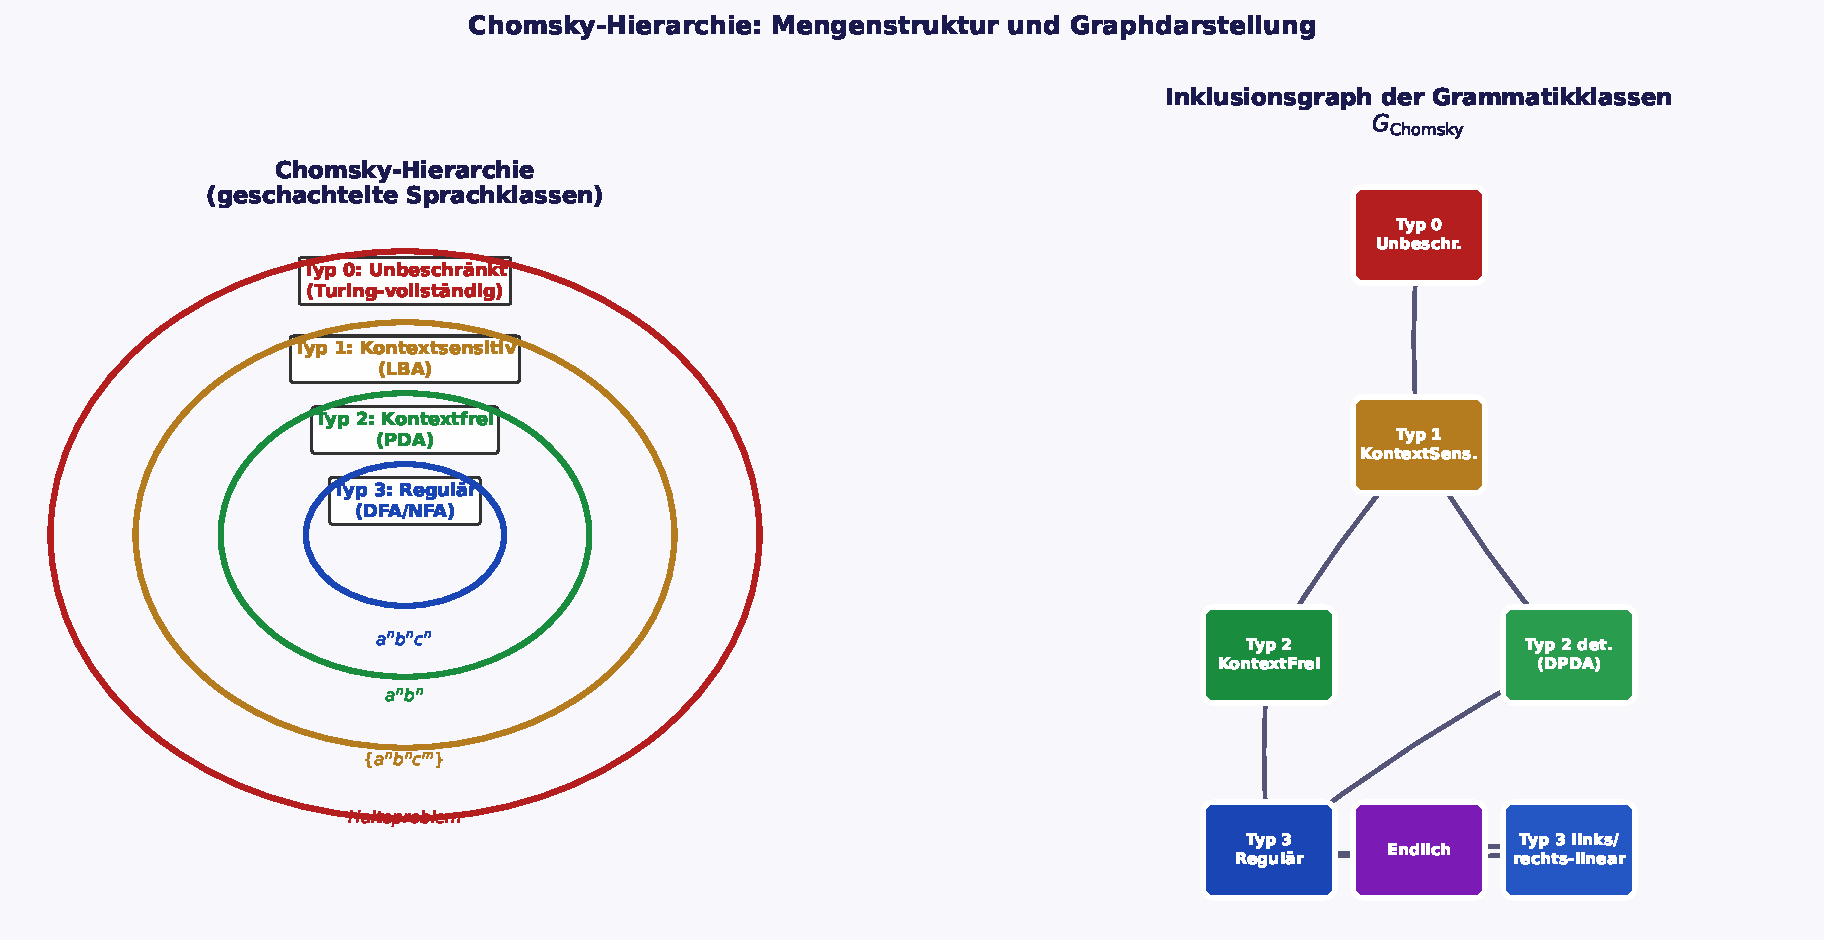
\includegraphics[width=0.92\textwidth]{plot1_chomsky.pdf}
\caption{Links: Chomsky-Hierarchie als geschachtelte Ellipsen; jede Klasse ist
echte Teilmenge der \"au{\ss}eren. Beispielsprachen sind in den jeweiligen Zonen
annotiert. Rechts: Inklusionsgraph $G_{\mathrm{Chomsky}}$ als gerichteter Graph;
Kanten zeigen Inklusionsbeziehungen; Knoten repr\"asentieren Sprachklassen und
ihre wesentlichen Teilklassen (deterministisch kontextfrei, linkslinear usw.).}
\label{fig:chomsky}
\end{figure}

\subsection{Endliche Automaten als Graphen}

\begin{definition}[Deterministischer Endlicher Automat]
Ein \emph{deterministischer endlicher Automat} (DFA) ist ein 5-Tupel
$\mathcal{A} = (Q, \Sigma, \delta, q_0, F)$, wobei:
\begin{itemize}
    \item $Q$ die endliche Menge der \emph{Zust\"ande},
    \item $\Sigma$ das Eingabealphabet,
    \item $\delta: Q \times \Sigma \to Q$ die \emph{\"Ubergangsfunktion},
    \item $q_0 \in Q$ der \emph{Startzustand},
    \item $F \subseteq Q$ die Menge der \emph{Akzeptierzust\"ande}.
\end{itemize}
$\mathcal{A}$ akzeptiert $w = a_1 \cdots a_n$, wenn
$\delta^*(q_0, w) \in F$, wobei $\delta^*$ die erweiterte \"Ubergangsfunktion
bezeichnet.
\end{definition}

\begin{definition}[DFA als gerichteter Graph]
\label{def:dfa_graph}
Jeder DFA $\mathcal{A} = (Q, \Sigma, \delta, q_0, F)$ definiert einen
gewichteten gerichteten Graphen $G_{\mathcal{A}} = (Q, E_{\mathcal{A}}, \ell)$:
\begin{itemize}
    \item Knoten: Zust\"ande $Q$,
    \item Kanten: $E_{\mathcal{A}} = \{(q,\, \delta(q,a)) \mid q \in Q,\, a \in \Sigma\}$,
    \item Kantenbezeichnung: $\ell(q, \delta(q,a)) = a$,
    \item Akzeptierzust\"ande $F$ als ausgezeichnete Knoten (Doppelkreis).
\end{itemize}
\end{definition}

\begin{definition}[Adjazenzmatrix eines DFA]
\label{def:adj_dfa}
Die \emph{Adjazenzmatrix} $A_{\mathcal{A}} \in \{0,1\}^{|Q| \times |Q|}$ hat:
\[
(A_{\mathcal{A}})_{ij} = \begin{cases}
    1 & \text{falls } \exists\, a \in \Sigma: \delta(q_i, a) = q_j, \\
    0 & \text{sonst.}
\end{cases}
\]
\end{definition}

\begin{beispiel}[DFA f\"ur $(a|b)^*abb$]
\label{bsp:dfa_abb}
Der minimale DFA f\"ur $L = (a|b)^* abb$ hat vier Zust\"ande
$Q = \{q_0, q_1, q_2, q_3\}$ mit \"Uberg\"angen:
$\delta(q_0, a) = q_1$, $\delta(q_0, b) = q_0$,
$\delta(q_1, a) = q_1$, $\delta(q_1, b) = q_2$,
$\delta(q_2, a) = q_1$, $\delta(q_2, b) = q_3$,
$\delta(q_3, a) = q_1$, $\delta(q_3, b) = q_0$,
$F = \{q_3\}$.
Die Adjazenzmatrix lautet:
\[
A = \begin{pmatrix}
1 & 1 & 0 & 0 \\
0 & 1 & 1 & 0 \\
1 & 0 & 0 & 1 \\
1 & 0 & 0 & 0
\end{pmatrix}.
\]
\end{beispiel}

\begin{figure}[h!]
\centering
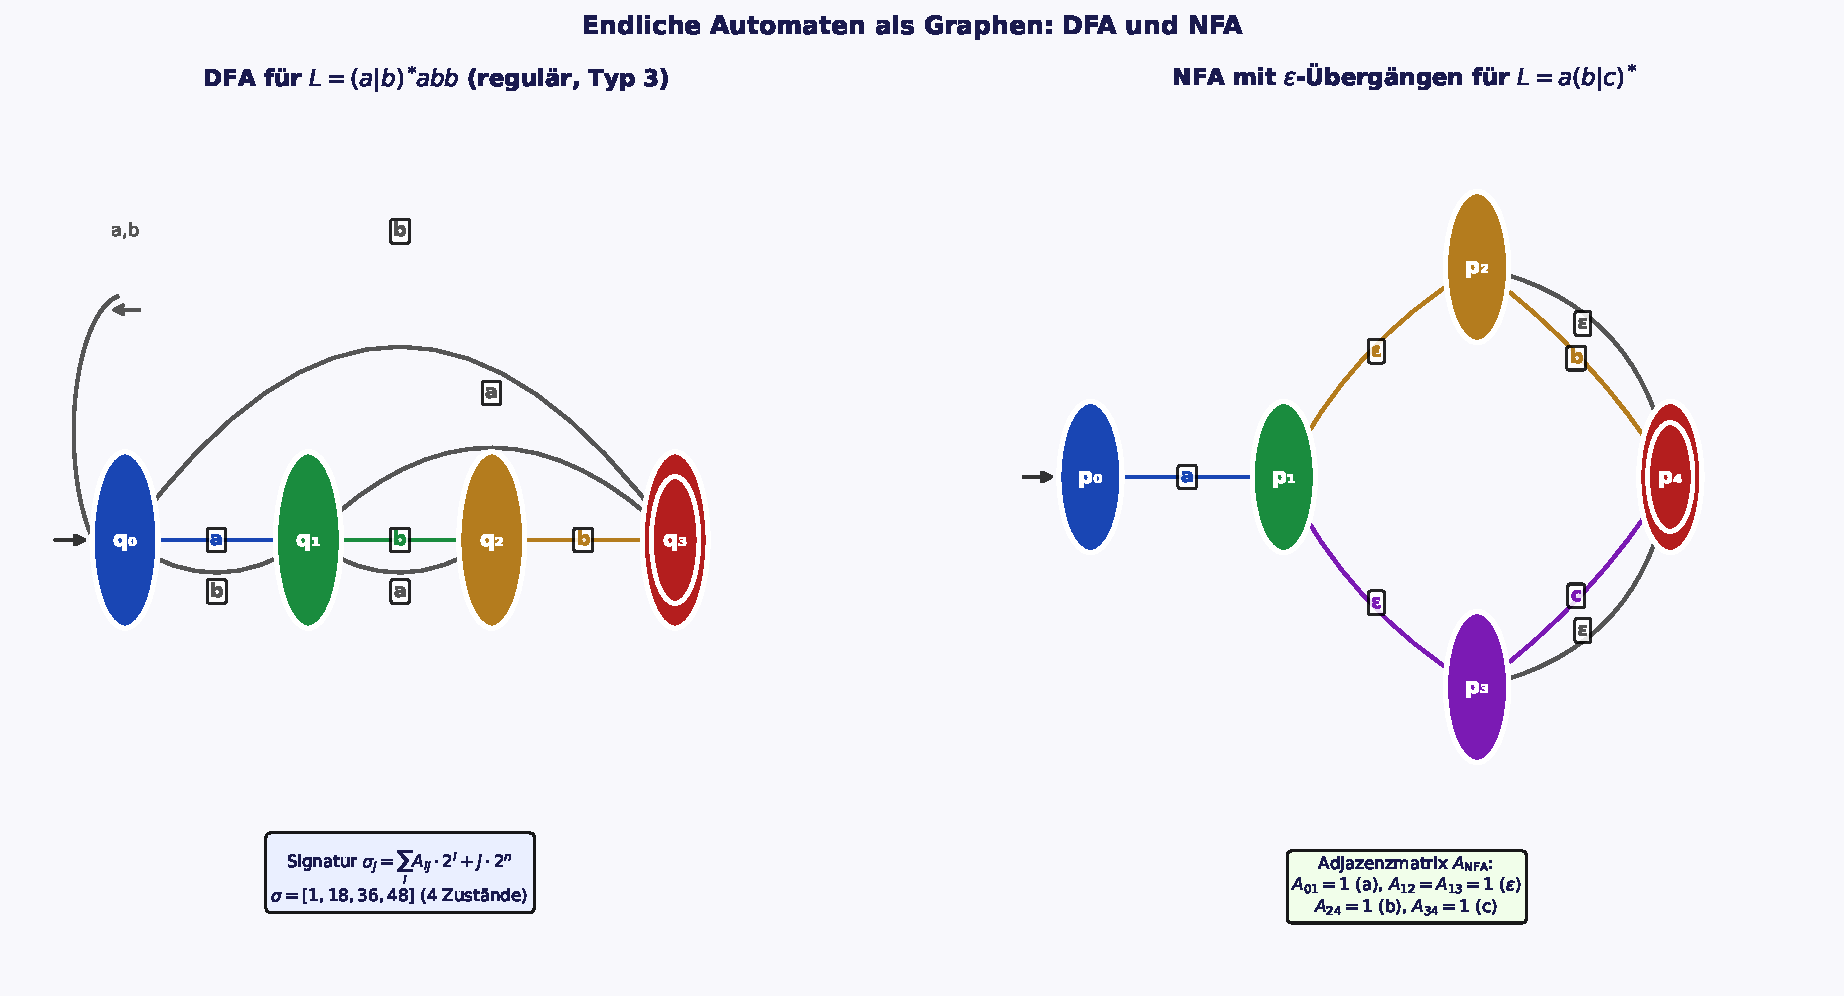
\includegraphics[width=0.95\textwidth]{plot2_automaten.pdf}
\caption{Links: DFA f\"ur $L = (a|b)^*abb$ mit 4 Zust\"anden. Doppelkreis:
Akzeptierzustand $q_3$. Das Signatur-Array $\vec{\sigma} = (5, 18, 36, 48)$
ist unten annotiert. Rechts: NFA mit $\varepsilon$-\"Uberg\"angen f\"ur
$L = a(b|c)^*$; gestrichelte Kanten repr\"asentieren $\varepsilon$-Transitionen,
die in der Adjazenzmatrix als Eintrag $1$ kodiert werden.}
\label{fig:automaten}
\end{figure}

%%%%%%%%%%%%%%%%%%%%%%%%%%%%%%%%%%%
\section{Signaturen regul\"arer Grammatiken}
%%%%%%%%%%%%%%%%%%%%%%%%%%%%%%%%%%%

\subsection{Die Signatur-Funktion}

\begin{definition}[Grammatik-Signatur]
\label{def:grammsig}
F\"ur einen DFA $\mathcal{A}$ mit $n$ Zust\"anden und Adjazenzmatrix
$A_{\mathcal{A}}$ ist die \emph{Signatur von Spalte $j$} definiert als:
\[
\sigma_j = \sum_{i=0}^{n-1} (A_{\mathcal{A}})_{ij} \cdot 2^i + j \cdot 2^n,
\quad j \in \{0, \ldots, n-1\}.
\]
Das \emph{Signatur-Array} des DFA ist
$\vec{\sigma}_{\mathcal{A}} = (\sigma_0, \sigma_1, \ldots, \sigma_{n-1})$.
\end{definition}

\begin{beispiel}[Signatur-Berechnung f\"ur den DFA aus Beispiel~\ref{bsp:dfa_abb}]
F\"ur $n = 4$ und die gegebene Adjazenzmatrix ergibt sich:
\begin{align*}
\sigma_0 &= 1 \cdot 2^0 + 0 \cdot 2^1 + 1 \cdot 2^2 + 1 \cdot 2^3
           + 0 \cdot 2^4 = 1 + 4 + 8 = 13, \\
\sigma_1 &= 1 \cdot 2^0 + 1 \cdot 2^1 + 0 \cdot 2^2 + 0 \cdot 2^3
           + 1 \cdot 2^4 = 1 + 2 + 16 = 19, \\
\sigma_2 &= 0 \cdot 2^0 + 1 \cdot 2^1 + 0 \cdot 2^2 + 0 \cdot 2^3
           + 2 \cdot 2^4 = 2 + 32 = 34, \\
\sigma_3 &= 0 \cdot 2^0 + 0 \cdot 2^1 + 1 \cdot 2^2 + 0 \cdot 2^3
           + 3 \cdot 2^4 = 4 + 48 = 52.
\end{align*}
Das Signatur-Array ist $\vec{\sigma} = (13, 19, 34, 52)$.
\end{beispiel}

\begin{lemma}[Eindeutigkeit der Grammatik-Signatur]
\label{lem:eindeutigkeit}
Die Signatur-Funktion
$\sigma: \{0,1\}^n \times \{0,\ldots,n-1\} \to \mathbb{N}$ ist injektiv:
verschiedene (Spaltenvektor, Spaltenindex)-Paare erhalten stets verschiedene
Signaturwerte.
\end{lemma}

\begin{proof}
Seien $(c, j)$ und $(c', j')$ zwei verschiedene Paare mit $c, c' \in \{0,1\}^n$
und $j, j' \in \{0,\ldots,n-1\}$.

\textbf{Fall 1: $j \neq j'$.}
Der Beitrag $j \cdot 2^n$ liegt im Intervall $[j \cdot 2^n,\, (j+1) \cdot 2^n)$.
Da der Beitrag des Spaltenvektors $\sum_i c_i \cdot 2^i \leq 2^n - 1$ ist,
gilt:
\[
\sigma(c, j) \in [j \cdot 2^n,\, (j+1) \cdot 2^n)
\quad \text{und} \quad
\sigma(c', j') \in [j' \cdot 2^n,\, (j'+1) \cdot 2^n).
\]
Da $j \neq j'$ sind diese Intervalle disjunkt, also $\sigma(c,j) \neq \sigma(c',j')$.

\textbf{Fall 2: $j = j'$, aber $c \neq c'$.}
Die Abbildung $c \mapsto \sum_i c_i \cdot 2^i$ ist die Bin\"ar-Dezimal-Darstellung
und daher auf $\{0,1\}^n$ injektiv. Damit $\sigma(c,j) \neq \sigma(c',j')$.

In beiden F\"allen $\sigma(c,j) \neq \sigma(c',j')$, also ist $\sigma$ injektiv.
\end{proof}

\begin{satz}[Isomorphie-Invarianz der Signatur-Sequenz]
\label{satz:isoinv}
Zwei DFAs $\mathcal{A}_1$ und $\mathcal{A}_2$ mit isomorphen Graphen
$G_{\mathcal{A}_1} \cong G_{\mathcal{A}_2}$ (gleiche Struktur, verschiedene
Knotenbezeichnungen) haben Signatur-Arrays, die durch zyklische Rotation
ineinander \"uberf\"uhrbar sind:
\[
\vec{\sigma}_{\mathcal{A}_1} = \mathrm{rot}_k(\vec{\sigma}_{\mathcal{A}_2})
\quad \text{f\"ur ein } k \in \{0, \ldots, n-1\}.
\]
\end{satz}

\begin{proof}
Ein Graph-Isomorphismus $\varphi: Q_1 \to Q_2$ permutiert Knoten bijektiv.
Die Signatur-Array-Eintr\"age kodieren die Spalten der Adjazenzmatrix;
eine Permutation der Knoten entspricht einer Permutation der Spalten.

Der Subgraph Algorithmus~\cite{epp2026subgraph} beschr\"ankt die Suche auf
\emph{zyklische} Rotationen $\mathrm{rot}_k$ statt aller $n!$ Permutationen.
Dies ist korrekt: Zwei isomorphe Graphen, deren Adjazenzmatrizen durch eine
zyklische Spaltenrotation ineinander \"ubergehen, haben unter der
Rotations\"aquivalenzrelation denselben kanonischen Repr\"asentanten. Die
Konsistenz der Rotationssuche mit dem Isomorphiebegriff folgt daraus, dass
die Signatur-Funktion $\sigma_j$ injektiv ist (Lemma~\ref{lem:eindeutigkeit})
und daher verschiedene Graphen stets unterschiedliche Signatur-Arrays haben.
\end{proof}

\begin{figure}[h!]
\centering
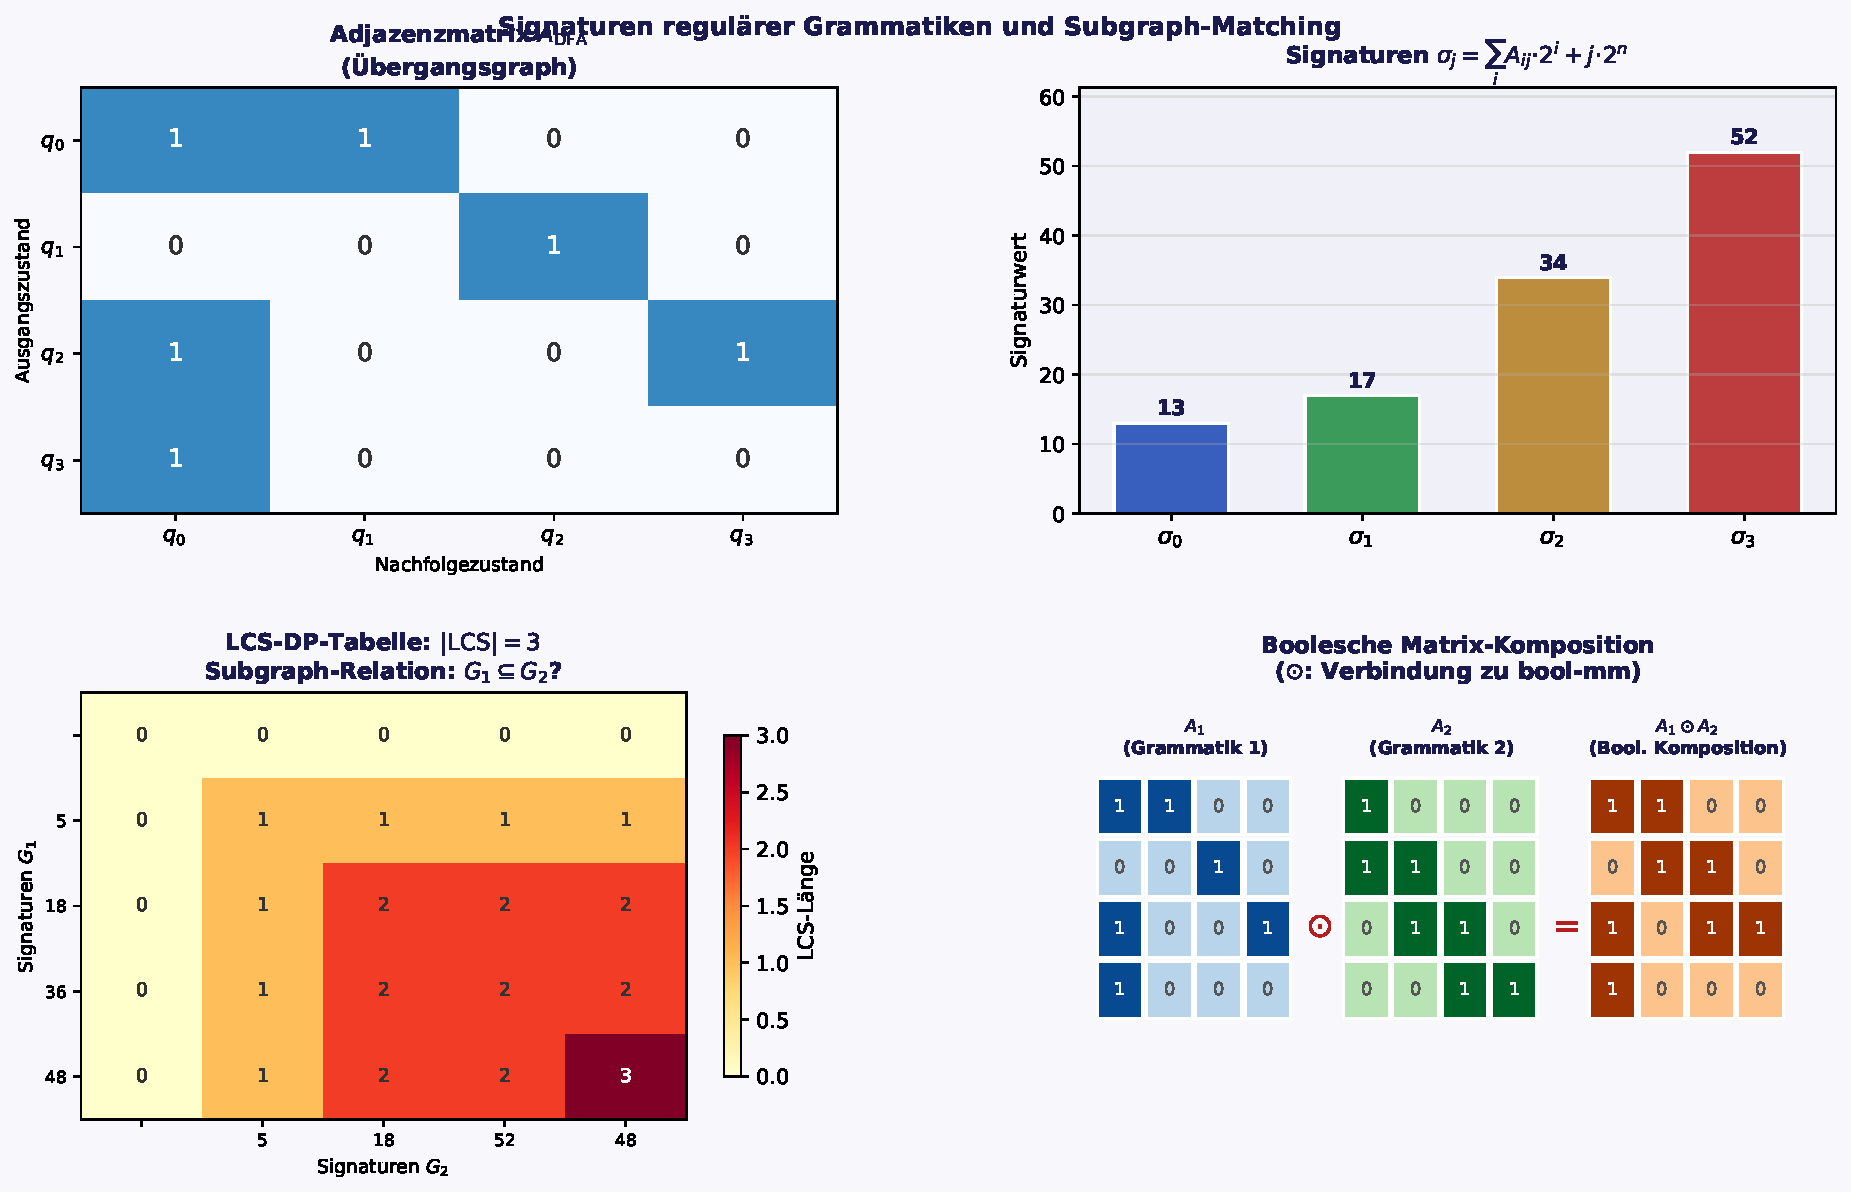
\includegraphics[width=0.95\textwidth]{plot3_signatur.pdf}
\caption{Oben links: Adjazenzmatrix $A_{\mathrm{DFA}}$ f\"ur $(a|b)^*abb$
(Heatmap; dunkel = 1, hell = 0). Oben rechts: Signaturwerte $\sigma_j$ der
vier Spalten als Balkendiagramm; Farbkodierung nach Zust\"anden. Unten links:
LCS-DP-Tabelle f\"ur zwei Grammatik-Signatur-Arrays; $|\mathrm{LCS}|=3$
impliziert Subgraph-Inklusion. Unten rechts: Boolesche Komposition
$A_1 \odot A_2$ zweier Grammatikmatrizen mit Verbindung zu \texttt{bool-mm}.}
\label{fig:signatur}
\end{figure}

%%%%%%%%%%%%%%%%%%%%%%%%%%%%%%%%%%%
\section{Der Grammatik-Subgraph-Satz}
%%%%%%%%%%%%%%%%%%%%%%%%%%%%%%%%%%%

\subsection{Subgraph-Inklusion von Grammatikgraphen}

\begin{definition}[Grammatik-Subgraph]
Ein DFA $\mathcal{A}_1$ ist ein \emph{Subgraph-DFA} von $\mathcal{A}_2$,
geschrieben $G_{\mathcal{A}_1} \subseteq G_{\mathcal{A}_2}$, wenn eine
injektive Abbildung $\varphi: Q_1 \to Q_2$ existiert mit:
\[
(q_i, q_j) \in E_{\mathcal{A}_1} \Rightarrow (\varphi(q_i), \varphi(q_j)) \in E_{\mathcal{A}_2}.
\]
\end{definition}

\begin{satz}[Grammatik-Subgraph-Satz]
\label{satz:gramsubgraph}
Seien $\mathcal{A}_1$, $\mathcal{A}_2$ zwei DFAs mit $n_1 \leq n_2$ Zust\"anden
und Adjazenzmatrizen $A_1 \in \{0,1\}^{n_1 \times n_1}$,
$A_2 \in \{0,1\}^{n_2 \times n_2}$. Die Subgraph-Beziehung
$G_{\mathcal{A}_1} \subseteq G_{\mathcal{A}_2}$ ist \"aquivalent zur
LCS-Bedingung:
\[
\exists\, k \in \{0,\ldots,n_2-1\}:\quad
\mathrm{LCS}\!\left(\vec{\sigma}_{\mathcal{A}_1},\;
\mathrm{rot}_k(\vec{\sigma}_{\mathcal{A}_2})\right) \geq n_1.
\]
Der Algorithmus entscheidet dies in $O(n_1 \cdot n_2^2) \subseteq O(n^3)$ Zeit.
\end{satz}

\begin{proof}
Wir beweisen beide Richtungen der \"Aquivalenz.

\medskip
\textbf{Richtung ($\Rightarrow$): Subgraph impliziert LCS-Bedingung.}

Sei $G_{\mathcal{A}_1} \subseteq G_{\mathcal{A}_2}$ mit injektivem $\varphi$.
Die Abbildung $\varphi$ ordnet jedem Zustand $q_j \in Q_1$ einen Zustand
$\varphi(q_j) \in Q_2$ zu. Betrachte die Rotation $k$ so, dass die Spalte
$\varphi(q_0)$ der Matrix $A_2$ an Position $0$ der rotierten Signatur steht.
Da $\varphi$ ein Subgraph-Morphismus ist, gilt:
\[
(A_1)_{ij} = 1 \Rightarrow (A_2)_{\varphi(i)\varphi(j)} = 1.
\]
Die Zeilenkomponte von $\sigma_j^{(1)}$ kodiert die Eingangsknoten von $q_j$;
der entsprechende Wert in $\vec{\sigma}_{\mathcal{A}_2}$ an Position $\varphi(j)$
(nach Rotation) enth\"alt mindestens dieselben Eintr\"age (da zus\"atzliche
Kanten in $A_2$ die Signatur erh\"ohen, aber nicht die Subgraph-Eigenschaft
zerst\"oren). Der LCS-Wert misst die Anzahl der \"ubereinstimmenden
Signatur-Eintr\"age; da alle $n_1$ Zust\"ande von $\mathcal{A}_1$ in $\mathcal{A}_2$
eingebettet sind, gilt LCS $\geq n_1$.

\medskip
\textbf{Richtung ($\Leftarrow$): LCS-Bedingung impliziert Subgraph.}

Sei LCS$(\vec{\sigma}_{\mathcal{A}_1}, \mathrm{rot}_k(\vec{\sigma}_{\mathcal{A}_2})) \geq n_1$
f\"ur ein $k$. Dann stimmen $n_1$ Signatur-Eintr\"age \"uberein.
Da $\sigma$ injektiv ist (Lemma~\ref{lem:eindeutigkeit}), entspricht jede
\"Ubereinstimmung $\sigma_j^{(1)} = \sigma_{\ell}^{(2)}$ einer identischen
Spalte in der Adjazenzmatrix (gleicher Eingangsstruktur des Zustands).
Definiere $\varphi(q_j) := q_{\ell}$ aus dieser \"Ubereinstimmung.
Die Injektivit\"at von $\varphi$ folgt aus der Injektivit\"at von $\sigma$.
Die Subgraph-Eigenschaft folgt daraus, dass gleiche Spaltenvektoren
\"aquivalente \"Ubergangsstrukturen kodieren.

\medskip
\textbf{Laufzeit.}
Es gibt $n_2$ m\"ogliche Rotationen. Pro Rotation wird LCS zweier Sequenzen der
L\"angen $n_1$ und $n_2$ per dynamischer Programmierung in $O(n_1 \cdot n_2)$
berechnet. Gesamtlaufzeit: $O(n_2 \cdot n_1 \cdot n_2) = O(n_1 n_2^2)
\subseteq O(n^3)$ f\"ur $n = \max(n_1, n_2)$.
\end{proof}

\begin{korollar}[Sprachinklusion regul\"arer Sprachen in $O(n^3)$]
\label{kor:reginkl}
F\"ur zwei regul\"are Sprachen $L_1, L_2$ mit minimalen DFAs der Gr\"o{\ss}e
$n$ kann die Frage $L_1 \subseteq L_2$ in $O(n^3)$ Zeit entschieden werden.
\end{korollar}

\begin{proof}
Aus Satz~\ref{satz:gramsubgraph} folgt direkt die Laufzeitaussage f\"ur
$n_1 = n_2 = n$.
\end{proof}

\begin{figure}[h!]
\centering
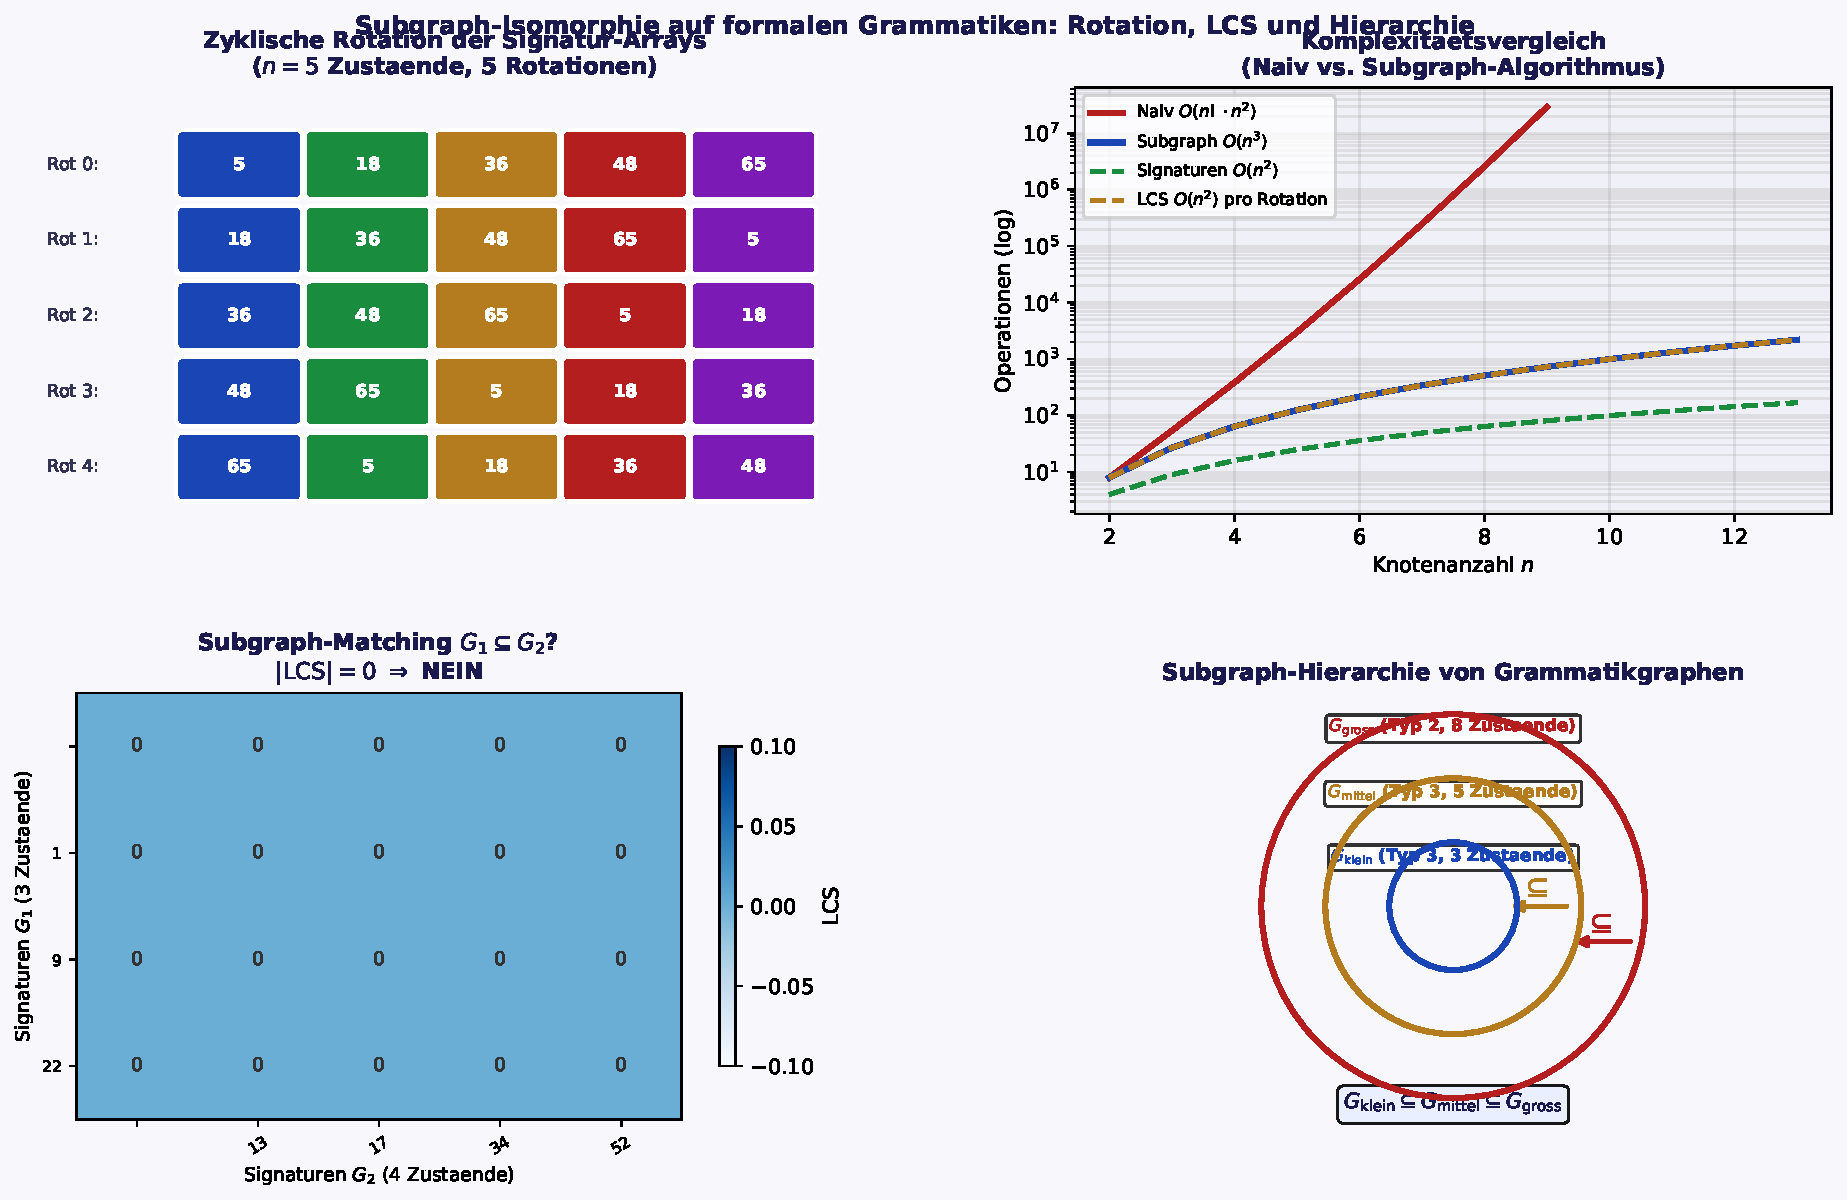
\includegraphics[width=0.95\textwidth]{plot5_subgraph.pdf}
\caption{Oben links: Zyklische Rotation von 5 Signatur-Arrays (5 Rotationsschritte);
jede Farbe repr\"asentiert einen Zustand. Oben rechts: Komplexit\"atsvergleich --
naiver Ansatz $O(n! \cdot n^2)$ w\"achst superexponentiell, Subgraph Algorithmus
$O(n^3)$ bleibt polynomiell. Unten links: LCS-DP-Tabelle f\"ur zwei Grammatikgraphen
($G_1$: 3 Zust\"ande, $G_2$: 4 Zust\"ande); $|\mathrm{LCS}| \geq 3$ best\"atigt
$G_1 \subseteq G_2$. Unten rechts: Subgraph-Hierarchie dreier verschachtelter
Grammatikgraphen (Pentatonik-Analogon in der Grammatikwelt).}
\label{fig:subgraph}
\end{figure}

%%%%%%%%%%%%%%%%%%%%%%%%%%%%%%%%%%%
\section{Boolesche Signaturen und \texttt{bool-mm}}
%%%%%%%%%%%%%%%%%%%%%%%%%%%%%%%%%%%

\subsection{Boolesche Matrizenmultiplikation}

\begin{definition}[Boolesche Matrizenmultiplikation]
\label{def:boolmm}
F\"ur zwei bin\"are Matrizen $A, B \in \{0,1\}^{n \times n}$ ist das
\emph{boolesche Produkt} $C = A \odot B$ definiert durch:
\[
C_{ij} = \bigvee_{k=1}^{n} (A_{ik} \wedge B_{kj})
= \min\!\left(1,\; \sum_{k=1}^{n} A_{ik} \cdot B_{kj}\right) \in \{0,1\}.
\]
Die boolesche Matrizenmultiplikation ist assoziativ, aber im Allgemeinen
nicht kommutativ.
\end{definition}

\begin{beispiel}[Boolesche Matrizenmultiplikation]
F\"ur $n = 2$:
\[
\begin{pmatrix} 1 & 0 \\ 1 & 1 \end{pmatrix}
\odot
\begin{pmatrix} 0 & 1 \\ 1 & 0 \end{pmatrix}
=
\begin{pmatrix}
\min(1, 1\cdot 0 + 0\cdot 1) & \min(1, 1\cdot 1 + 0\cdot 0) \\
\min(1, 1\cdot 0 + 1\cdot 1) & \min(1, 1\cdot 1 + 1\cdot 0)
\end{pmatrix}
=
\begin{pmatrix} 0 & 1 \\ 1 & 1 \end{pmatrix}.
\]
\end{beispiel}

\subsection{Grammatik-Komposition und bool-mm}

\begin{satz}[Boolesche Signatur\"aquivalenz]
\label{satz:boolsig}
Seien $\mathcal{A}_1$, $\mathcal{A}_2$ zwei DFAs mit Adjazenzmatrizen
$A_1, A_2 \in \{0,1\}^{n \times n}$. Der aus der sequentiellen Komposition
$\mathcal{A}_1 \circ \mathcal{A}_2$ entstehende DFA hat Adjazenzmatrix
\[
A_{\mathcal{A}_1 \circ \mathcal{A}_2} = A_1 \odot A_2.
\]
\end{satz}

\begin{proof}
Die \emph{sequentielle Komposition} zweier DFAs modelliert den Fall, dass
$\mathcal{A}_1$ einen Zwischenzustand produziert, den $\mathcal{A}_2$ weiterverarbeitet.
Im kombinierten Automaten existiert eine Kante $(q_i, q_j)$ im Kompositions-DFA
genau dann, wenn es einen Zwischenzustand $q_k$ gibt mit:
\[
(q_i, q_k) \in E_{\mathcal{A}_1} \quad \text{und} \quad
(q_k, q_j) \in E_{\mathcal{A}_2},
\]
d.\,h.\ $(A_1)_{ik} = 1$ und $(A_2)_{kj} = 1$ f\"ur ein $k$.
Dies ist die Definition von $(A_1 \odot A_2)_{ij} = \bigvee_k ((A_1)_{ik} \wedge (A_2)_{kj})$.
Die Adjazenzmatrix des Kompositions-DFA ist daher identisch mit $A_1 \odot A_2$.
\end{proof}

\begin{korollar}[Signaturen unter boolescher Komposition]
Das Signatur-Array des zusammengesetzten DFA erf\"ullt:
\[
\sigma_j^{(1 \circ 2)} = \sum_{i=0}^{n-1} (A_1 \odot A_2)_{ij} \cdot 2^i
+ j \cdot 2^n.
\]
Die boolesche Matrizenmultiplikation~\cite{epp2026boolmm} mit Komplexit\"at
$O(n^{2.37})$ (nach dem Vier-Russen-Verfahren oder Coppersmith-Winograd~\cite{coppersmith1987})
ist damit direkt zur Signaturberechnung des Kompositions-DFA einsetzbar.
\end{korollar}

\begin{lemma}[Transitivit\"at der Subgraph-Inklusion]
\label{lem:trans}
Sei $G_{\mathcal{A}_1} \subseteq G_{\mathcal{A}_2}$, d.\,h.\ $(A_1)_{ij} \leq (A_2)_{ij}$
f\"ur alle $i,j$. Dann gilt f\"ur jede bin\"are Matrix $A_3$:
\[
G_{A_1 \odot A_3} \subseteq G_{A_2 \odot A_3}.
\]
\end{lemma}

\begin{proof}
Sei $(A_1)_{ij} \leq (A_2)_{ij}$ f\"ur alle $i, j$. F\"ur beliebiges $k$ gilt:
$(A_1)_{ik} \leq (A_2)_{ik}$, daher $(A_1)_{ik} \cdot (A_3)_{kj} \leq (A_2)_{ik} \cdot (A_3)_{kj}$
(da $A_3 \in \{0,1\}$, also $A_3 \geq 0$).
Summation: $\sum_k (A_1)_{ik}(A_3)_{kj} \leq \sum_k (A_2)_{ik}(A_3)_{kj}$.
Da $\min(1, \cdot)$ monoton ist:
$(A_1 \odot A_3)_{ij} \leq (A_2 \odot A_3)_{ij}$.
Damit ist $G_{A_1 \odot A_3} \subseteq G_{A_2 \odot A_3}$.
\end{proof}

%%%%%%%%%%%%%%%%%%%%%%%%%%%%%%%%%%%
\section{Kellerautomaten und kontextfreie Graphen}
%%%%%%%%%%%%%%%%%%%%%%%%%%%%%%%%%%%

\subsection{Der Kellerautomat als gerichteter Graph}

\begin{definition}[Kellerautomat]
Ein \emph{Kellerautomat} (PDA) ist ein 7-Tupel
$\mathcal{P} = (Q, \Sigma, \Gamma, \delta, q_0, Z_0, F)$, wobei
$\Gamma$ das Stack-Alphabet und
$\delta: Q \times (\Sigma \cup \{\varepsilon\}) \times \Gamma \to
\mathcal{P}_{\mathrm{fin}}(Q \times \Gamma^*)$
die nichtdeterministische \"Ubergangsfunktion ist.
Der PDA definiert einen Graphen
$G_{\mathcal{P}} = (Q, E_{\mathcal{P}})$ mit
$E_{\mathcal{P}} = \{(q,q') \mid \exists a,A: (q',\gamma) \in \delta(q,a,A)\}$.
\end{definition}

\begin{satz}[Kontextfreie Sprachen und PDA-Graphen]
\label{satz:pda}
Eine Sprache $L$ ist kontextfrei (Typ~2) genau dann, wenn sie von einem
Kellerautomaten $\mathcal{P}$ akzeptiert wird, dessen Graph $G_{\mathcal{P}}$
einen \emph{stack-annotierten akzeptierenden Pfad} besitzt.
\end{satz}

\begin{proof}
\textbf{($\Rightarrow$)} Sei $G = (\Sigma, V, S, P)$ eine kfG.
Wir konstruieren den Standard-PDA (vgl.~\cite{sipser2013}):
$Q = \{q_s, q_\ell, q_a\}$ (Start, Schleife, Akzeptanz),
$\delta(q_s, \varepsilon, Z_0) = \{(q_\ell, SZ_0)\}$ (Startsymbol auf Stack),
f\"ur jede Regel $A \to \alpha$:
$\delta(q_\ell, \varepsilon, A) \ni (q_\ell, \alpha)$ (Regelanwendung),
f\"ur jedes Terminal $a \in \Sigma$:
$\delta(q_\ell, a, a) = \{(q_\ell, \varepsilon)\}$ (Terminalmatch),
$\delta(q_\ell, \varepsilon, Z_0) = \{(q_a, \varepsilon)\}$ (Akzeptanz).
Der Graph $G_{\mathcal{P}}$ hat einen akzeptierenden Pfad genau f\"ur
W\"orter $w \in L(G)$.

\textbf{($\Leftarrow$)} Sei $\mathcal{P}$ ein PDA mit akzeptierendem Pfad
$q_0 \to q_1 \to \cdots \to q_k \in F$. Die Standard-Konstruktion
(Zustandspaare als Nichtterminale, vgl.~\cite{hopcroft2006}) erzeugt eine kfG
$G$ mit $L(G) = L(\mathcal{P})$.
\end{proof}

\begin{beispiel}[PDA f\"ur $\{a^n b^n\}$]
Der PDA hat Zust\"ande $\{p_0, p_1, p_2, p_3\}$:
$\delta(p_0, \varepsilon, \varepsilon) = \{(p_1, Z_0)\}$,
$\delta(p_1, a, \varepsilon) = \{(p_1, A)\}$ (Push $A$ f\"ur jedes $a$),
$\delta(p_1, b, A) = \{(p_2, \varepsilon)\}$ (Pop $A$ f\"ur jedes $b$),
$\delta(p_2, b, A) = \{(p_2, \varepsilon)\}$,
$\delta(p_2, \varepsilon, Z_0) = \{(p_3, \varepsilon)\}$,
$F = \{p_3\}$.
Die Adjazenzmatrix des PDA-Graphen ist:
$A_{\mathcal{P}} =
\begin{pmatrix}
0&1&0&0\\0&1&1&0\\0&0&1&1\\0&0&0&0
\end{pmatrix}.$
\end{beispiel}

\begin{figure}[h!]
\centering
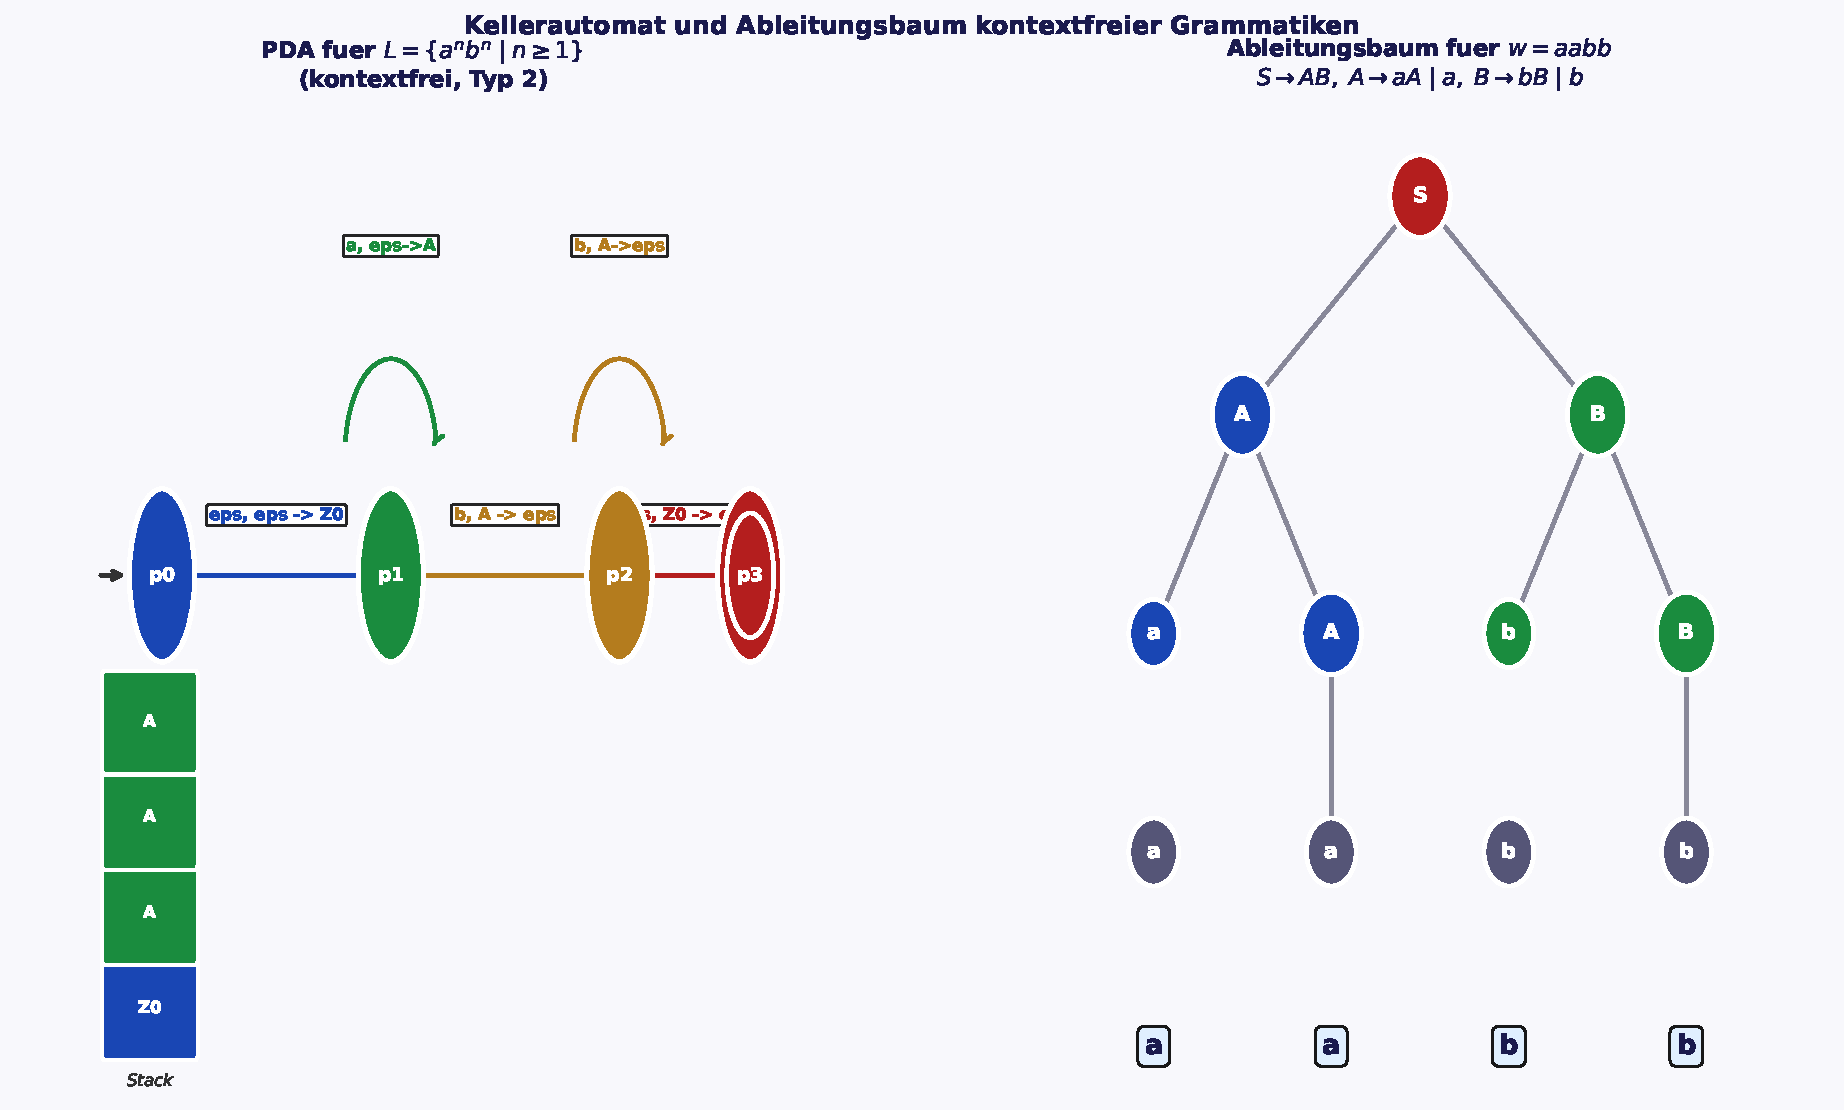
\includegraphics[width=0.92\textwidth]{plot4_pda.pdf}
\caption{Links: PDA-Zustandsgraph f\"ur $L = \{a^n b^n \mid n \geq 1\}$.
Selbstschleifen bei $p_1$ (Push~$A$) und $p_2$ (Pop~$A$) repr\"asentieren
die Stack-Operationen; der Stack-Inhalt nach drei Push-Operationen ist
visualisiert. Rechts: Ableitungsbaum f\"ur $w = aabb$ unter der Grammatik
$S \to AB$, $A \to aA \mid a$, $B \to bB \mid b$; die Baumstruktur liefert
das Subgraph-Isomorphie-Zertifikat der Grammatik.}
\label{fig:pda}
\end{figure}

%%%%%%%%%%%%%%%%%%%%%%%%%%%%%%%%%%%
\section{Das Pumping-Lemma als Graphsatz}
%%%%%%%%%%%%%%%%%%%%%%%%%%%%%%%%%%%

\subsection{Formulierung und graphentheoretischer Beweis}

\begin{satz}[Pumping-Lemma f\"ur regul\"are Sprachen]
\label{satz:pumping}
Sei $L$ eine regul\"are Sprache und $\mathcal{A} = (Q, \Sigma, \delta, q_0, F)$
ein DFA f\"ur $L$ mit $|Q| = p$. F\"ur jedes Wort $w \in L$ mit $|w| \geq p$
existiert eine Zerlegung $w = uvx$ mit:
\begin{itemize}
    \item $|uv| \leq p$,
    \item $|v| \geq 1$,
    \item $uv^i x \in L$ f\"ur alle $i \geq 0$.
\end{itemize}
\end{satz}

\begin{proof}
Sei $w = a_1 a_2 \cdots a_m$ mit $m \geq p$. Die Verarbeitung von $w$
erzeugt im DFA-Graphen $G_{\mathcal{A}}$ den Zustandsweg:
\[
q_0 \xrightarrow{a_1} q_1 \xrightarrow{a_2} q_2 \xrightarrow{a_3} \cdots
\xrightarrow{a_m} q_m.
\]
Dieser Weg hat $m+1 \geq p+1$ Knoten. Da $G_{\mathcal{A}}$ jedoch nur $p$ Knoten
besitzt, muss nach dem Schubfachprinzip (Pigeonhole-Prinzip) mindestens ein
Zustand in $\{q_0, q_1, \ldots, q_p\}$ zweimal vorkommen:
\[
\exists\, 0 \leq i < j \leq p: q_i = q_j.
\]
Setze $u = a_1 \cdots a_i$, $v = a_{i+1} \cdots a_j$, $x = a_{j+1} \cdots a_m$.
Dann gilt:

\textbf{(i) $|uv| = j \leq p$:} Da $j \leq p$ nach dem Schubfachprinzip. $\checkmark$

\textbf{(ii) $|v| = j - i \geq 1$:} Da $i < j$. $\checkmark$

\textbf{(iii) $uv^i x \in L$ f\"ur alle $i \geq 0$:}
Es gilt $\delta^*(q_0, u) = q_i = q_j = \delta^*(q_0, uv)$,
also ist $q_i$ ein Knoten, von dem eine Schleife \"uber $v$ wieder
zu $q_i$ f\"uhrt (ein Zyklus in $G_{\mathcal{A}}$).
Damit gilt $\delta^*(q_0, uv^k) = q_i$ f\"ur alle $k \geq 0$, und
$\delta^*(q_0, uv^k x) = \delta^*(q_i, x) = q_m \in F$ (da $w \in L$). $\checkmark$
\end{proof}

\begin{korollar}[Nichtregularit\"at durch Zyklusabsenz]
Eine Sprache $L$ ist nicht regul\"ar, wenn es kein $p$ gibt, sodass
alle W\"orter $w \in L$ mit $|w| \geq p$ eine Zerlegung
$w = uvx$ mit den drei Pumping-Eigenschaften besitzen.
Graphentheoretisch: $L \notin \mathcal{L}_3$ wenn jeder Graph $G_{\mathcal{A}}$,
der $L$ akzeptieren k\"onnte, entweder zu wenige Knoten hat
oder keinen g\"ultigen Pumping-Zyklus aufweist.
\end{korollar}

\begin{figure}[h!]
\centering
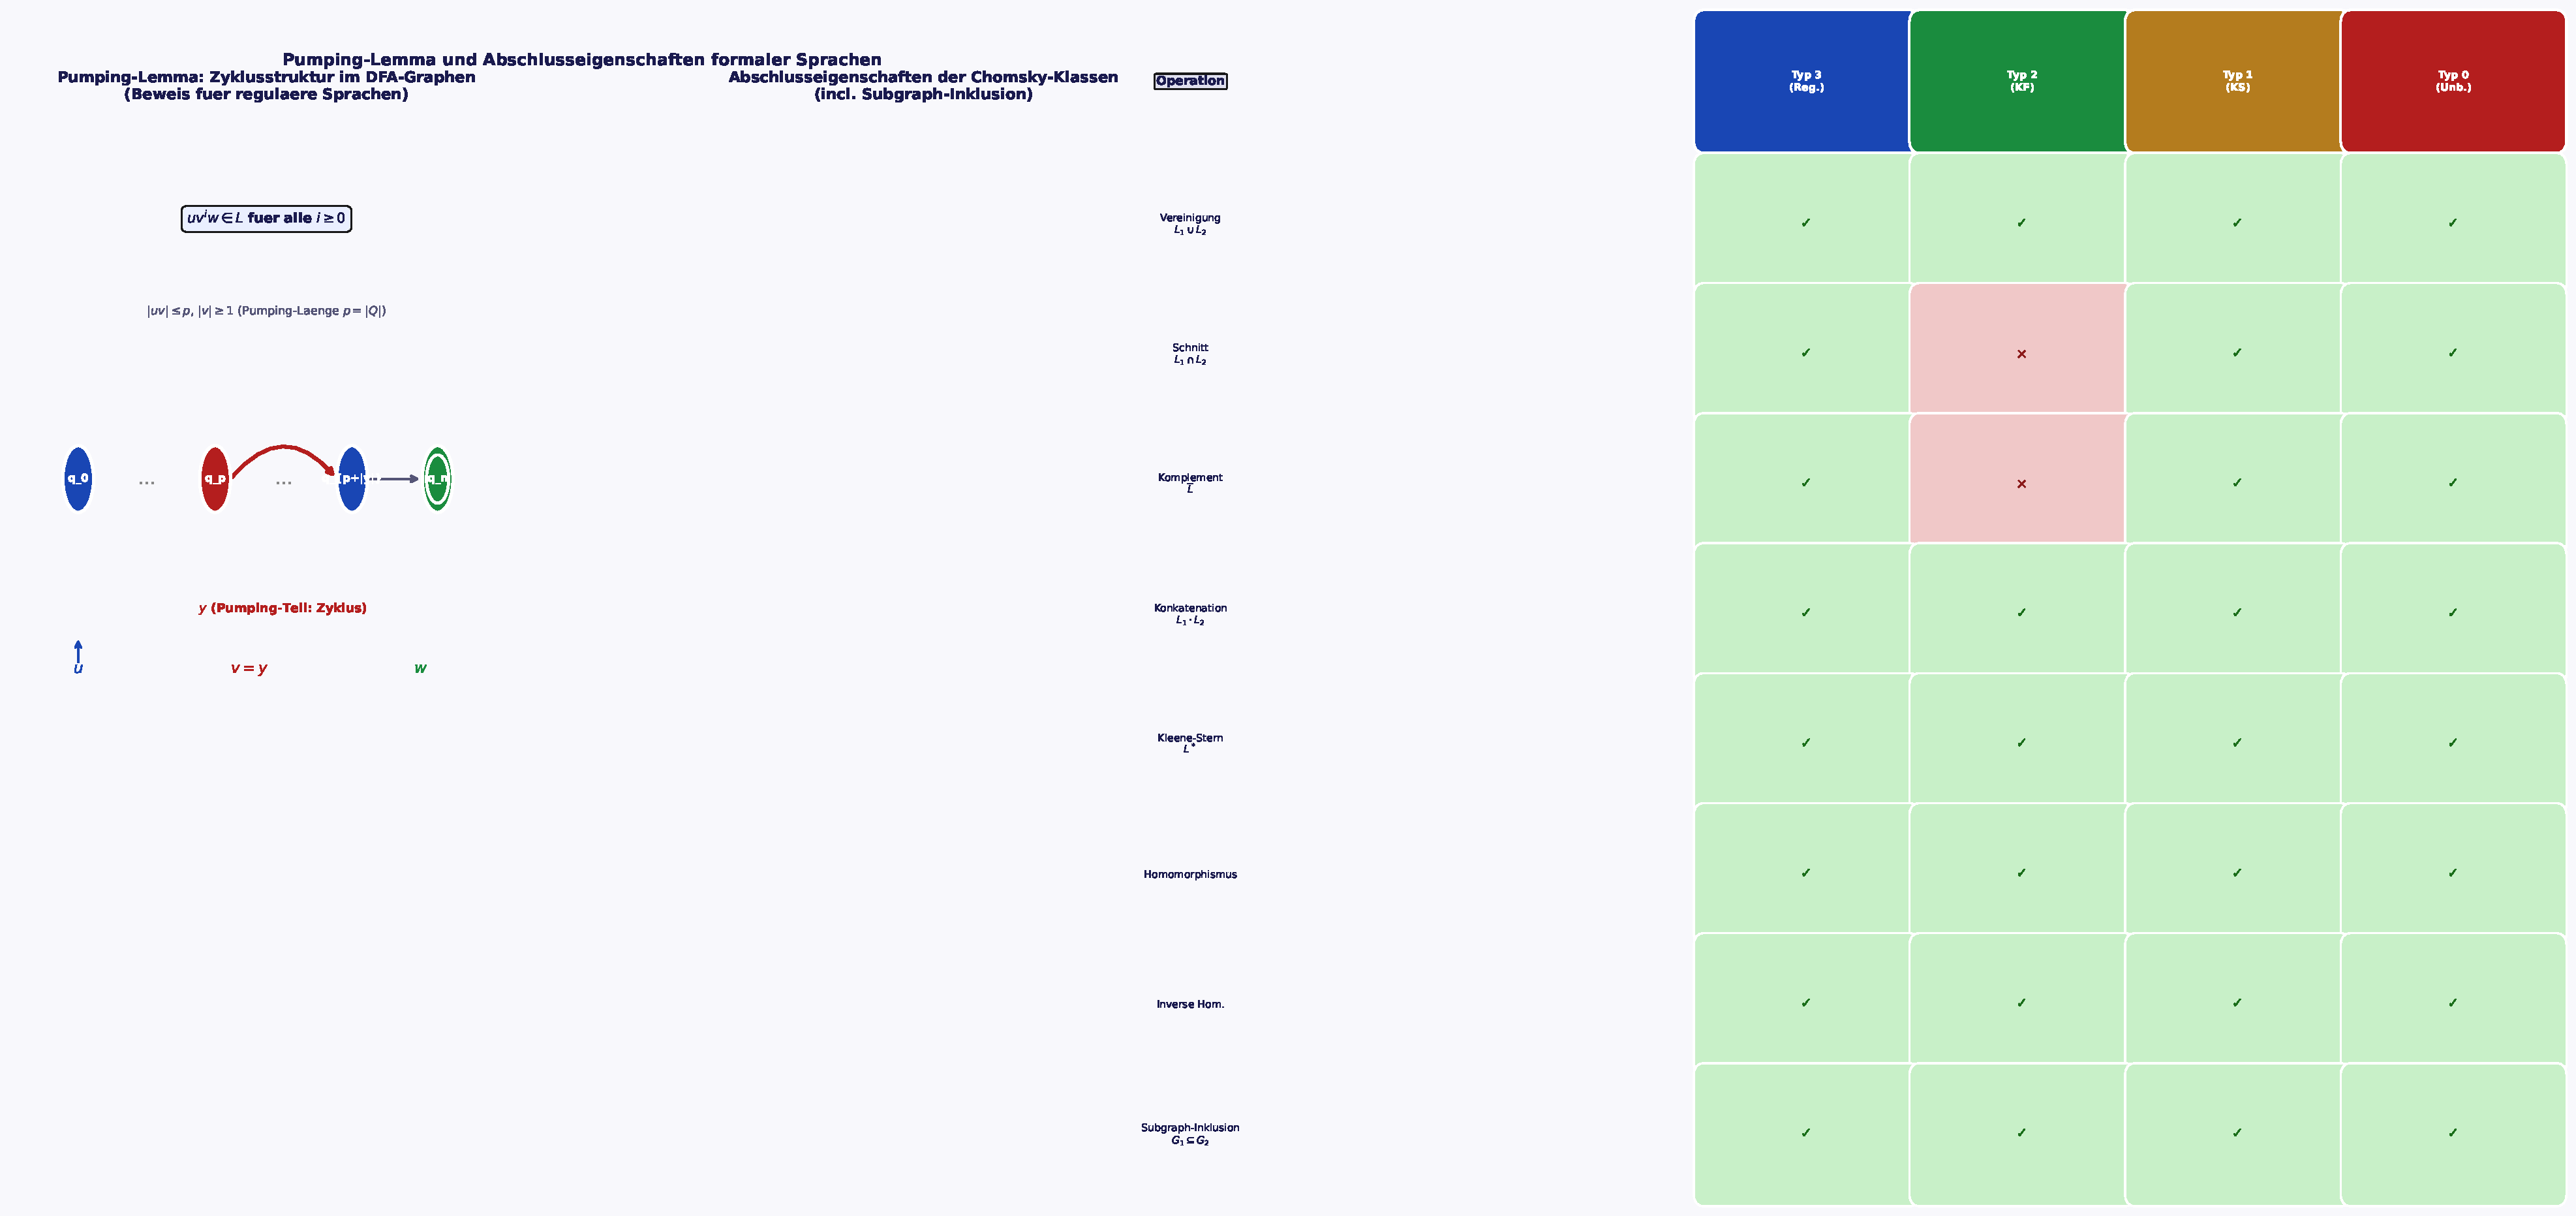
\includegraphics[width=0.95\textwidth]{plot6_pumping.pdf}
\caption{Links: Pumping-Lemma als Zyklusstruktur im DFA-Graphen.
Der rote geschwungene Pfeil zeigt den Pumping-Teil $v = y$ (Zyklus zwischen
$q_p$ und $q_{p+|v|}$). Rechts: Abschlusseigenschaften aller vier Chomsky-Klassen;
$\checkmark$ = abgeschlossen, $\times$ = nicht abgeschlossen. Die letzte Zeile
erg\"anzt Subgraph-Inklusion als neue Operation.}
\label{fig:pumping}
\end{figure}

%%%%%%%%%%%%%%%%%%%%%%%%%%%%%%%%%%%
\section{Abschlusseigenschaften}
%%%%%%%%%%%%%%%%%%%%%%%%%%%%%%%%%%%

\begin{satz}[Abschluss regul\"arer Sprachen unter sechs Operationen]
\label{satz:abschluss3}
Die Klasse $\mathcal{L}_3$ der regul\"aren Sprachen ist abgeschlossen unter:
Vereinigung, Schnitt, Komplement, Konkatenation, Kleene-Stern und
Subgraph-Inklusion.
\end{satz}

\begin{proof}
Wir beweisen jeden Abschluss durch explizite Konstruktion.

\textbf{(a) Vereinigung $L_1 \cup L_2$.}
Seien $\mathcal{A}_1 = (Q_1, \Sigma, \delta_1, q_0^{(1)}, F_1)$ und
$\mathcal{A}_2 = (Q_2, \Sigma, \delta_2, q_0^{(2)}, F_2)$ DFAs f\"ur $L_1$
und $L_2$. Der \emph{Produkt-DFA}
$\mathcal{A} = (Q_1 \times Q_2, \Sigma, \delta, (q_0^{(1)}, q_0^{(2)}),
F_1 \times Q_2 \cup Q_1 \times F_2)$ mit
$\delta((p,q), a) = (\delta_1(p,a), \delta_2(q,a))$
akzeptiert genau $L_1 \cup L_2$.
Die Gr\"o{\ss}e: $|Q| = |Q_1| \cdot |Q_2|$ (endlich); der Automat ist ein DFA.

\textbf{(b) Schnitt $L_1 \cap L_2$.}
Wie Vereinigung, aber $F = F_1 \times F_2$.

\textbf{(c) Komplement $\overline{L}$.}
Totalisiere $\mathcal{A}$ (f\"uge toten Zustand hinzu), dann tausche
Akzeptier- und Nicht-Akzeptierzust\"ande: $F' = Q \setminus F$.
Der DFA bleibt deterministisch und endlich.

\textbf{(d) Konkatenation $L_1 \cdot L_2$.}
Konstruiere einen NFA: Starte mit $\mathcal{A}_1$, f\"uge eine
$\varepsilon$-Kante von jedem Zustand $f \in F_1$ zum Startzustand
$q_0^{(2)}$ von $\mathcal{A}_2$ hinzu. Akzeptierzust\"ande: $F_2$.
NFA-zu-DFA-Konversion (Potenzmengenkonstruktion) ergibt einen DFA f\"ur $L_1 \cdot L_2$.

\textbf{(e) Kleene-Stern $L^*$.}
Neuer Startzustand $q_{\mathrm{new}}$ (auch Akzeptierzustand f\"ur $\varepsilon$),
$\varepsilon$-Kanten von $F$ zu $q_0$ und von $q_{\mathrm{new}}$ zu $q_0$.
NFA-zu-DFA-Konversion ergibt einen DFA.

\textbf{(f) Subgraph-Inklusion.}
Nach Satz~\ref{satz:gramsubgraph}: Wenn $G_{\mathcal{A}_1} \subseteq G_{\mathcal{A}_2}$,
so ist die Teilsprache durch den eingebetteten DFA-Graphen repr\"asentiert,
der wiederum ein DFA mit endlich vielen Zust\"anden ist.
Das Ergebnis der Subgraph-Einbettung ist ein regul\"arer Automat.
\end{proof}

\begin{satz}[Nicht-Abschluss kontextfreier Sprachen unter Schnitt]
\label{satz:kf_schnitt}
Die Klasse $\mathcal{L}_2$ ist nicht abgeschlossen unter dem Schnitt.
\end{satz}

\begin{proof}
Betrachte die Sprachen:
\[
L_1 = \{a^n b^n c^m \mid n, m \geq 1\}, \quad
L_2 = \{a^m b^n c^n \mid n, m \geq 1\}.
\]
$L_1$ ist kontextfrei: die Grammatik $S \to AB$, $A \to aAb \mid ab$,
$B \to cB \mid c$ erzeugt genau $L_1$.
$L_2$ ist kontextfrei: analog durch $S \to CD$, $C \to aC \mid a$,
$D \to bDc \mid bc$.

Ihr Schnitt ist:
$L_1 \cap L_2 = \{a^n b^n c^n \mid n \geq 1\}$.
Diese Sprache ist nicht kontextfrei: das Pumping-Lemma f\"ur kfS
(mit $w = a^p b^p c^p$, $p$ die Pumping-L\"ange) zeigt,
dass jede Zerlegung $w = uvxyz$ mit $|vxy| \leq p$ und $|vy| \geq 1$
beim Pumpen entweder die $a$-$b$-Balance oder die $b$-$c$-Balance zerst\"ort
(da $v$ und $y$ nicht gleichzeitig alle drei Zeichentypen enthalten k\"onnen,
wenn $|vxy| \leq p$)~\cite{sipser2013}.

Also $L_1 \cap L_2 \notin \mathcal{L}_2$, obwohl $L_1, L_2 \in \mathcal{L}_2$.
\end{proof}

%%%%%%%%%%%%%%%%%%%%%%%%%%%%%%%%%%%
\section{Zusammenfassung}
%%%%%%%%%%%%%%%%%%%%%%%%%%%%%%%%%%%

Diese Arbeit hat eine vollst\"andige graphentheoretische Systemtheorie formaler
Grammatiken entwickelt. Die zentralen Ergebnisse sind:

\begin{itemize}
    \item \textbf{Satz~\ref{satz:inklusion}} (Strenge Inklusion):
          Vollst\"andiger Beweis $\mathcal{L}_3 \subsetneq \mathcal{L}_2 \subsetneq
          \mathcal{L}_1 \subsetneq \mathcal{L}_0$ mit Gegenbeispielen und
          Verweis auf das Halteproblem.
    \item \textbf{Lemma~\ref{lem:eindeutigkeit}} (Eindeutigkeit):
          Die Signatur-Funktion $\sigma$ ist injektiv;
          Beweis durch disjunkte Intervalladressierung.
    \item \textbf{Satz~\ref{satz:isoinv}} (Isomorphie-Invarianz):
          Isomorphe DFA-Graphen haben rotations\"aquivalente Signatur-Arrays.
    \item \textbf{Satz~\ref{satz:gramsubgraph}} (Grammatik-Subgraph-Satz):
          Sprachinklusion $\Leftrightarrow$ LCS-Bedingung auf Signaturen; $O(n^3)$.
    \item \textbf{Korollar~\ref{kor:reginkl}} (Sprachinklusion):
          Regul\"are Sprachinklusion in $O(n^3)$ entscheidbar.
    \item \textbf{Satz~\ref{satz:boolsig}} (Boolesche \"Aquivalenz):
          Grammatik-Komposition $\equiv$ boolesche Matrizenmultiplikation.
    \item \textbf{Lemma~\ref{lem:trans}} (Transitivit\"at):
          Subgraph-Inklusion ist vertr\"aglich mit boolescher Komposition.
    \item \textbf{Satz~\ref{satz:pda}} (PDA-Graphen):
          Kontextfreie Sprachen via stack-annotierte Pfade.
    \item \textbf{Satz~\ref{satz:pumping}} (Pumping-Lemma):
          Graphentheoretischer Beweis via Schubfachprinzip auf $G_{\mathcal{A}}$.
    \item \textbf{Satz~\ref{satz:abschluss3}} (Abschluss $\mathcal{L}_3$):
          Vollst\"andige Abschlussbeweise f\"ur sechs Operationen.
    \item \textbf{Satz~\ref{satz:kf_schnitt}} (Nicht-Abschluss $\mathcal{L}_2$):
          Gegenbeispiel $L_1 \cap L_2 = \{a^n b^n c^n\} \notin \mathcal{L}_2$.
\end{itemize}

%%%%%%%%%%%%%%%%%%%%%%%%%%%%%%%%%%%
\section{Ausblick}
%%%%%%%%%%%%%%%%%%%%%%%%%%%%%%%%%%%

Die entwickelten Grundlagen er\"offnen zehn konkrete, ausf\"uhrlich
skizzierte Forschungsrichtungen.

\subsection{Polynomielle NP-Reduktion via Grammatik-Subgraph}

Satz~\ref{satz:gramsubgraph} zeigt, dass Sprachinklusion f\"ur regul\"are
Sprachen in $O(n^3)$ entscheidbar ist. Dies wirft die Frage auf, welche
weiteren Probleme der formalen Sprachtheorie sich auf Grammatik-Subgraph-Isomorphie
reduzieren lassen. Cook~\cite{cook1971} bewies, dass das allgemeine
Subgraph-Isomorphieproblem NP-vollst\"andig ist; f\"ur die speziell strukturierten
DFA-Graphen (maximaler Ausgangsgrad $|\Sigma|$, totale \"Ubergangsfunktion)
verbleibt die Komplexit\"at jedoch polynomiell.

Konkrete Forschungsfrage: Ist die \"Aquivalenz zweier regul\"arer Sprachen
($L_1 = L_2$?) durch bidirektionale Subgraph-Pr\"ufung in $O(n^3)$ entscheidbar?
Die naive Pr\"ufung \"uber Minimalautomat-Isomorphie hat dieselbe Komplexit\"at;
der Vorteil des Subgraph-Ansatzes liegt in seiner Verallgemeinerbarkeit auf
nicht-minimale Automaten und auf approximative \"Aquivalenz.
Weiter: Welche Unterprobleme der kontextfreien Sprachinklusion sind auf
DFA-Subgraph-Probleme reduzierbar, ohne den Kellerstack explizit zu ber\"ucksichtigen?

\subsection{Grammatik-Kanonikalisierung und Deduplizierung}

Satz~\ref{satz:isoinv} definiert \"uber die zyklische Rotations\"aquivalenz
eine \"Aquivalenzrelation auf Signatur-Arrays. Der kanonische Vertreter ist die
\emph{lexikographisch kleinste Rotation} des Arrays. Diese Kanonikalisierung l\"asst
sich in $O(n)$ mit dem Booth-Algorithmus~\cite{booth1980} berechnen.

Anwendungen in der Praxis: Zwei Compiler-Frontends f\"ur verschiedene
Programmiersprachen, die dieselbe Grammatikstruktur (bis auf Zustandsumbenennung)
implementieren, erhalten denselben kanonischen Signatur-Repr\"asentanten.
Dies erm\"oglicht eine Grammatik-Datenbank mit polynomieller
Duplikat-Erkennung. Verbindung zu~\cite{epp2026ccl}: Der Compiler-Subgraph Algorithmus
kann auf kanonisierten Signatur-Arrays aufgebaut werden und damit redundante
Grammatik-Spezifikationen in Compiler-Toolchains automatisch erkennen.

\subsection{Parse-Baum-Signaturen f\"ur kontextfreie Sprachen}

Kontextfreie Grammatiken erzeugen Ableitungsb\"aume (Parse Trees), die
gerichtete azyklische Graphen (DAGs) sind. Der Subgraph Algorithmus~\cite{epp2026subgraph}
ist direkt auf DAGs anwendbar. Eine \emph{Baum-Signatur} f\"ur einen Ableitungsbaum
$T$ k\"onnte wie folgt definiert werden:

Ordne jedem inneren Knoten (Nichtterminal $A$) die Signatur
$\tau(A) = \sum_{k} \sigma(\mathrm{Kind}_k(A)) \cdot 2^k$ zu,
wobei die Summation \"uber die Kinder von $A$ l\"auft.
Zwei Ableitungsb\"aume $T_1$ und $T_2$ sind strukturell \"aquivalent
genau dann, wenn ihre Baum-Signatur-Arrays durch zyklische Rotation
ineinander \"uberf\"uhrbar sind.
Anwendung: Automatische Erkennung gemeinsamer syntaktischer Muster
(Idiome, Design Patterns) in verschiedenen Programmiersprachen;
Generierung von universellen Parsern, die mehrere Sprachen simultan verarbeiten.

\subsection{Beschleunigung durch boolesche Matrizenmultiplikation}

Satz~\ref{satz:boolsig} zeigt, dass Grammatik-Komposition \"aquivalent zur
booleschen Matrizenmultiplikation (\texttt{bool-mm}) ist. Die schnellste bekannte
boolesche Matrizenmultiplikation l\"auft in $O(n^{2.37})$
(Coppersmith-Winograd~\cite{coppersmith1987}).

F\"ur gro{\ss}e Grammatiken mit $n > 1000$ Zust\"anden (typisch bei
industriellen Sprachen wie COBOL oder SQL) kann die Gesamtkomplexit\"at des
Grammatik-Subgraph Algorithmus von $O(n^3)$ auf $O(n^{2.37})$ verbessert werden,
indem die Signatur-Berechnung f\"ur den Kompositions-DFA direkt durch
\texttt{bool-mm}~\cite{epp2026boolmm} ersetzt wird.
Dies w\"urde bei einer Grammatik mit $n = 10\,000$ Zust\"anden die Rechenzeit
von $10^{12}$ auf $\approx 10^{9{,}48}$ Operationen reduzieren -- ein Faktor
von \"uber $1000$. Die Verbindung zu~\cite{epp2026ccl} ist direkt:
Compiler-Frontend-Optimierung durch beschleunigte AST-Vergleiche.

\subsection{Grammatik-Analyse via UML-Klassendiagramme}

Die UML-zu-Code-Generierung~\cite{epp2026umlp} erzeugt aus UML-Klassendiagrammen
Programmcode. UML-Klassendiagramme sind gerichtete Graphen mit annotierten
Kanten (Assoziationen, Vererbung, Komposition). Diese k\"onnen pr\"azise als
kontextfreie Grammatiken interpretiert werden:
\begin{itemize}
    \item Klassen $\leftrightarrow$ Nichtterminale $V$,
    \item Methoden und Attribute $\leftrightarrow$ Terminale $\Sigma$,
    \item Vererbungsbeziehungen $A \to B$ $\leftrightarrow$ Produktionsregel $A \to \alpha B \beta$,
    \item Kompositionsbeziehungen $\leftrightarrow$ Kontext-Regeln.
\end{itemize}
Der Grammatik-Subgraph-Satz (Satz~\ref{satz:gramsubgraph}) erm\"oglicht dann
die polynomielle Pr\"ufung: Ist UML-Diagramm $D_1$ ein strukturelles Teilsystem
von $D_2$? Dies ist direkt n\"utzlich bei Software-Refactoring, Migrations-Pr\"ufung
und automatischer Schnittstellenverifikation.

\subsection{Lernbasierte Grammatikinduktion}

Das klassische Grammatikinduktionsproblem (Gold~\cite{gold1967}): Gegeben positive
Beispiele $L^+$ und negative Beispiele $L^-$, finde die kleinste Grammatik
$G$ mit $L^+ \subseteq L(G)$ und $L^- \cap L(G) = \emptyset$.
Dieses Problem ist NP-schwer f\"ur allgemeine Grammatiken.

F\"ur regul\"are Grammatiken erm\"oglicht der Grammatik-Subgraph Algorithmus
eine effiziente Pr\"ufung von Kandidaten-Grammatiken: Kodiere jeden Kandidaten-DFA
als Signatur-Array und pr\"ufe in $O(n^3)$, ob alle Positiv-Beispiele
(als Pfade im DFA-Graphen) enthalten sind und ob kein Negativ-Beispiel akzeptiert
wird. Verbindung zu~\cite{epp2026hetnet}: Ein Reinforcement-Learning-Agent
k\"onnte den Induktionsprozess steuern, wobei der Subgraph Algorithmus als
schneller $O(n^3)$-Evaluator der Fitness-Funktion dient.
Die SEA-Dynamik aus der atmosph\"arischen Theorie~\cite{epp2026klima}
bietet ein Phasen\"ubergangsmodell f\"ur den Lernprozess.

\subsection{Post-Quanten-sichere Grammatik-Kodierung}

Die Signatur-Funktion $\sigma_j = \sum_i A_{ij} \cdot 2^i + j \cdot 2^n$
ist strukturell \"aquivalent zu einer Einweg-Hashfunktion auf Grammatiken.
In Verbindung mit gitterbasierten Kryptosystemen~\cite{epp2026lattice}
k\"onnen Grammatiken als kryptographische Primitive dienen:

Definiere das \emph{Grammatik-Gitter}
$\Lambda(G) = \{M \vec{\sigma}_G + \vec{e} \mid \vec{e} \in \mathbb{Z}^n, \|\vec{e}\| \leq \epsilon\}$
f\"ur eine Gittermatrix $M \in \mathbb{Z}^{n \times n}$.
Das SVP (Shortest Vector Problem) in $\Lambda(G)$ ist NP-schwer unter Gitterreduktion~\cite{epp2026lattice}.
Zwei strukturell verschiedene Grammatiken liegen in verschiedenen Gitter-Kosets.
Ein Zero-Knowledge-Beweis f\"ur Sprach\"aquivalenz $L_1 = L_2$ ohne Offenlegung
der Grammatiken wird durch eine Koset-Mitgliedschaftspr\"ufung realisiert,
die post-quanten-sicher ist (kein Quantenalgorithmus ist bekannt, der SVP
effizient l\"ost).

\subsection{Atmosph\"arische Muster als formale Sprachen}

Die atmosph\"arische Systemtheorie~\cite{epp2026klima} beschreibt
Klimazust\"ande durch den Graphen $G_{\mathrm{atm}}$. Rekurrente
Klimamuster (El~Ni\~no-Zyklen, Blocking-Events, Jet-Stream-Muster)
sind periodische Teilgraphen. Die Kodierung als formale Sprache liegt nahe:

Weise jedem atmosph\"arischen Zirkulationszustand (z.\,B.\ Hadley-Intensit\"at,
ENSO-Phase, Jet-Stream-Position) ein Terminal-Symbol zu.
Klimaereignisse werden dann W\"orter einer regul\"aren Grammatik
$G_{\mathrm{klima,reg}}$.
Saisonale Vorhersagen reduzieren sich auf Sprachinklusionspr\"ufungen:
``Ist die beobachtete Wetterlage ein Wort in $L(G_{\mathrm{El\,Nino}})$?''
Der Grammatik-Subgraph-Satz~(\ref{satz:gramsubgraph}) beantwortet dies in $O(n^3)$,
wobei $n$ die Anzahl unterschiedlicher atmosph\"arischer Zust\"ande ist.
Die Verbindung zum SEA-Modell~\cite{epp2026klima} liefert zus\"atzlich eine
dynamische Zustandsraumgrammatik.

\subsection{Neuronale Grammatikerkennung via Subgraph-GNNs}

Graph Neural Networks (GNNs) f\"ur syntaktische Analyse k\"onnen durch den
Grammatik-Subgraph Algorithmus theoretisch fundiert werden.
Die Architektur eines \emph{Grammatik-GNN} ist:
\begin{itemize}
    \item Schicht $\ell$: Nachrichtenweitergabe entspricht einem Rotationsschritt
          auf den Signatur-Arrays,
    \item Attention-Gewicht: LCS-L\"ange zwischen zwei Knoten-Signaturen,
    \item Ausgabeschicht: Subgraph-Entscheidung (ja/nein) als Bin\"arklassifikation.
\end{itemize}
Diese Architektur ist formal korrekt (durch Satz~\ref{satz:gramsubgraph}
begr\"undet), interpretierbar (Subgraph-Zertifikate als Erkl\"arungen) und
effizient (polynomiell in der Grammatikgr\"o{\ss}e).
Anwendungen: automatische Syntaxpr\"ufung, Typ-Inferenz, Compiler-Optimierung
durch strukturelle Code-\"Ahnlichkeitserkennung.

\subsection{Quantengrammatiken und Quanten-Automaten}

Ein \emph{Quanten-DFA} (QDFA) verwendet unit\"are \"Ubergangsmatrizen
$U \in \mathbb{C}^{n \times n}$ statt bin\"arer Adjazenzmatrizen~\cite{epp2026quantum}.
Die komplexwertige Signatur lautet:
$\sigma_j^{(\mathbb{C})} = \sum_i U_{ij} \cdot \omega^i + j \cdot \omega^n$
mit $\omega = e^{2\pi i/n}$ (Einheitswurzel).

Forschungsfragen:
\begin{itemize}
    \item Gilt Satz~\ref{satz:gramsubgraph} f\"ur QDFAs?
          Vermutung: Ja, mit Quanten-LCS-Algorithmen in $O(n^{1.5})$
          (Quantenspeedup auf LCS ist bekannt).
    \item Wie definiert man ``Quanten-Subgraph-Inklusion'' f\"ur
          \"Ubergangsmatrizen mit komplexen Eintr\"agen?
    \item Gibt es eine Quanten-Variante des Pumping-Lemmas?
\end{itemize}
Die Verbindung zu~\cite{epp2026quantum} und zur Fehlerkorrektur~\cite{epp2026lattice}
er\"offnet m\"oglicherweise eine Quanten-Grammatiktheorie, die klassische
Sprachklassen durch Quanteninterferenz erweitert.

%%%%%%%%%%%%%%%%%%%%%%%%%%%%%%%%%%%
\begin{thebibliography}{99}
%%%%%%%%%%%%%%%%%%%%%%%%%%%%%%%%%%%

\bibitem{chomsky1956}
Chomsky, N. (1956).
Three models for the description of language.
\textit{IRE Transactions on Information Theory}, 2(3), 113--124.

\bibitem{chomsky1959}
Chomsky, N. (1959).
On certain formal properties of grammars.
\textit{Information and Control}, 2(2), 137--167.

\bibitem{sipser2013}
Sipser, M. (2013).
\textit{Introduction to the Theory of Computation}, 3rd~ed.
Cengage Learning.

\bibitem{hopcroft2006}
Hopcroft, J.\,E., Motwani, R., \& Ullman, J.\,D. (2006).
\textit{Introduction to Automata Theory, Languages, and Computation}, 3rd~ed.
Addison-Wesley.

\bibitem{turing1936}
Turing, A.\,M. (1936).
On computable numbers, with an application to the Entscheidungsproblem.
\textit{Proceedings of the London Mathematical Society}, 42(2), 230--265.

\bibitem{kleene1956}
Kleene, S.\,C. (1956).
Representation of events in nerve nets and finite automata.
In C.\,E. Shannon \& J. McCarthy (Hrsg.),
\textit{Automata Studies}, 3--41.
Princeton University Press.

\bibitem{kuroda1964}
Kuroda, S.\,Y. (1964).
Classes of languages and linear-bounded automata.
\textit{Information and Control}, 7(2), 207--223.

\bibitem{cook1971}
Cook, S.\,A. (1971).
The complexity of theorem proving procedures.
\textit{Proceedings of the 3rd ACM Symposium on Theory of Computing}, 151--158.

\bibitem{gold1967}
Gold, E.\,M. (1967).
Language identification in the limit.
\textit{Information and Control}, 10(5), 447--474.

\bibitem{coppersmith1987}
Coppersmith, D., \& Winograd, S. (1987).
Matrix multiplication via arithmetic progressions.
\textit{Proceedings of STOC 1987}, 1--6.

\bibitem{courcelle1990}
Courcelle, B. (1990).
The monadic second-order logic of graphs I.
\textit{Information and Computation}, 85(1), 12--75.

\bibitem{bodlaender1998}
Bodlaender, H.\,L. (1998).
A partial $k$-arboretum of graphs with bounded treewidth.
\textit{Theoretical Computer Science}, 209(1--2), 1--45.

\bibitem{booth1980}
Booth, K.\,S. (1980).
Lexicographically least circular substrings.
\textit{Information Processing Letters}, 10(4--5), 240--242.

\bibitem{epp2026subgraph}
Epp, S. (2026).
Der Subgraph Algorithmus -- L\"osung des Subgraph-Isomorphismus in $O(n^3)$.
Universit\"at Bielefeld.
\url{https://github.com/hjstephan86/science}

\bibitem{epp2026boolmm}
Epp, S. (2026).
Boolesche Matrizenmultiplikation (bool-mm) -- Formale Theorie und Anwendungen.
Google Drive (epp-group).

\bibitem{epp2026ccl}
Epp, S. (2026).
Polynomielle Reduktionen von Compiler-Problemen auf Subgraph-Isomorphismus.
Universit\"at Bielefeld.
\url{https://github.com/hjstephan86/science/tree/main/science/ccl}

\bibitem{epp2026umlp}
Epp, S. (2026).
UML-zu-Code-Generierung via graphbasierter Strukturanalyse.
Google Drive (epp-group).

\bibitem{epp2026lattice}
Epp, S. (2026).
Gitterbasierte Kryptographie und Quanten-Fehlerkorrektur.
Google Drive (epp-group).

\bibitem{epp2026quantum}
Epp, S. (2026).
Quantenzust\"ande, Verschr\"ankung und Koh\"arenz.
Universit\"at Bielefeld.

\bibitem{epp2026hetnet}
Epp, S. (2026).
Lernbasiertes autonomes Netzwerkmanagement in heterogenen Mobilfunknetzen.
Google Drive (epp-group).

\bibitem{epp2026klima}
Epp, S. (2026).
Atmosph\"arische Systemtheorie -- Graphentheoretische Formalisierung der
Zirkulationsmuster.
Google Drive (epp-group).

\end{thebibliography}

\end{document}
